% =====================================================================
%  DOST-SEI SCHOLARSHIP EXAM REVIEWER  (Undergraduate Scholarship Examination)
%  Part I  : Creative Reasoning (Mechanical, Spatial, Verbal) + Language & Literature
%  Part II : Science (Biology, Chemistry, Earth Science, Physics, Space Science)
%  Part III: Mathematics (Algebra, Geometry, Trigonometry, Statistics, Calculus)
%  + Primer sample items explained, 100-item Mock Exam, Answer Sheet, Key & Solutions
%
%  Unofficial student reviewer. Not affiliated with or endorsed by DOST-SEI.
%  Exam structure, timing, and sample items: 2026 DOST-SEI Undergraduate
%  Scholarship Examination Primer. Older item styles: DOST-SEI
%  "SYENSIYA-bilidad: Developing One's Skills in Test-taking" (2013).
%  Every mock-exam question and passage in this file is original.
%
%  Paper : short bond paper (US Letter, 8.5 in x 11 in)
%  Build : pdfLaTeX, XeLaTeX, LuaLaTeX, or Tectonic (works on Overleaf)
% =====================================================================
\documentclass[10pt]{article}

% ---------- Page setup: short bond paper, tight margins ----------
\usepackage[letterpaper, top=0.55in, bottom=0.55in, left=0.5in, right=0.5in,
            headheight=14pt, headsep=5pt, footskip=16pt]{geometry}

% ---------- Fonts and math ----------
\usepackage[T1]{fontenc}
\usepackage{lmodern}
\usepackage{amsmath, amssymb}
\usepackage{pifont}

% ---------- Graphics, boxes, tables, lists ----------
\usepackage[dvipsnames, table]{xcolor}
\usepackage{graphicx}
\usepackage{tikz}
\usetikzlibrary{arrows.meta, calc, positioning, decorations.pathreplacing}
\usepackage[most]{tcolorbox}
\usepackage{array, tabularx, booktabs}
\usepackage{multicol}
\usepackage{enumitem}
\usepackage{fancyhdr}
\usepackage[hidelinks]{hyperref}

% ---------- Iskolar ng Agham palette ----------
\definecolor{dnavy}{HTML}{0B2D5B}
\definecolor{dblue}{HTML}{0D6EBD}
\definecolor{dsky}{HTML}{29ABE2}
\definecolor{dice}{HTML}{E6F2FB}
\definecolor{dmist}{HTML}{F3F8FD}
\definecolor{dgold}{HTML}{F2B01E}
\definecolor{palegold}{HTML}{FFF6E0}
\definecolor{rosered}{HTML}{C8324B}
\definecolor{palerose}{HTML}{FCEBEE}
\definecolor{dgreen}{HTML}{1E8C4E}
\definecolor{palegreen}{HTML}{EAF6EE}

% ---------- Paragraphs and lists ----------
\setlength{\parindent}{0pt}
\setlength{\parskip}{2pt}
\setlength{\columnsep}{0.22in}
\setlength{\columnseprule}{0.3pt}
\def\columnseprulecolor{\color{dblue!25}}
\setlist{itemsep=0pt, topsep=1pt, parsep=0.5pt, partopsep=0pt}
\setlist[itemize,1]{label={\color{dsky}\scriptsize$\blacksquare$}, leftmargin=1.1em}
\setlist[itemize,2]{label={\color{dsky}\scriptsize$\triangleright$}, leftmargin=1.0em}
\setlist[enumerate,1]{leftmargin=1.3em, label={\color{dblue}\bfseries\arabic*.}}
\renewcommand{\tabularxcolumn}[1]{p{#1}}
\renewcommand{\arraystretch}{1.12}
\newcolumntype{L}{>{\raggedright\arraybackslash}X}

% ---------- Little atom (used in headings and the title) ----------
\newcommand{\atom}[1][white]{\tikz[baseline=-0.6ex]{%
  \draw[#1, line width=0.55pt] (0,0) ellipse (0.19 and 0.065);
  \draw[#1, line width=0.55pt, rotate=60] (0,0) ellipse (0.19 and 0.065);
  \draw[#1, line width=0.55pt, rotate=120] (0,0) ellipse (0.19 and 0.065);
  \fill[#1] (0,0) circle (0.035);}}

% ---------- Chemistry and units ----------
\newcommand{\chem}[1]{\ensuremath{\mathrm{#1}}}
\newcommand{\yields}{\ensuremath{\rightarrow}}

% ---------- Header and footer ----------
\pagestyle{fancy}
\fancyhf{}
\fancyhead[L]{\scriptsize\sffamily\color{dblue}\textbf{DOST-SEI Scholarship Exam Reviewer} \,|\, Iskolar ng Agham}
\fancyhead[R]{\scriptsize\sffamily\color{dblue}Creative Reasoning \textbullet\ Language \& Literature \textbullet\ Science \textbullet\ Mathematics}
\fancyfoot[C]{\scriptsize\sffamily\color{gray}\thepage}
\fancyfoot[R]{\tiny\sffamily\color{gray}Unofficial student reviewer \textbullet\ not affiliated with DOST-SEI}
\renewcommand{\headrulewidth}{0.6pt}
\renewcommand{\headrule}{\hbox to\headwidth{\color{dgold}\leaders\hrule height \headrulewidth\hfill}}
\fancypagestyle{firstpage}{\fancyhf{}\fancyfoot[C]{\scriptsize\sffamily\color{gray}\thepage}%
  \fancyfoot[R]{\tiny\sffamily\color{gray}Unofficial student reviewer \textbullet\ not affiliated with DOST-SEI}%
  \renewcommand{\headrulewidth}{0pt}}

% ---------- Headings (never left alone at the bottom of a column) ----------
\raggedcolumns
\makeatletter
\newcommand{\sect}[2]{\par\vspace{3pt}%
  \begin{tcolorbox}[enhanced, colback=dblue, colframe=dblue, boxrule=0pt, arc=2pt,
    left=5pt, right=5pt, top=1.5pt, bottom=1.5pt, before skip=2pt, after={\par\nobreak},
    fontupper=\sffamily\bfseries\normalsize, coltext=white]
  \atom[dgold]\enspace{\color{dgold}#1}\enspace #2
  \end{tcolorbox}\nobreak\vspace{3pt}\nobreak\@afterheading}
\newcommand{\sub}[1]{\par\vspace{2.5pt}{\sffamily\bfseries\color{dblue}#1}\par\nobreak\vspace{0.5pt}\@afterheading}
\makeatother
\newcommand{\term}[1]{\textbf{\color{dnavy}#1}}
\newcommand{\no}{\textcolor{rosered}{\ding{55}}}
\newcommand{\yes}{\textcolor{dgreen}{\ding{51}}}

% ---------- Boxes ----------
\newtcolorbox{keybox}[1][Remember]{enhanced, colback=palegold, colframe=dgold,
  boxrule=0pt, leftrule=3pt, sharp corners, left=5pt, right=5pt, top=2pt, bottom=2pt,
  before skip=3pt, after skip=3pt,
  before upper={{\sffamily\bfseries\color{dgold!55!black}#1.}\ }}
\newtcolorbox{caution}[1][Trap]{enhanced, colback=palerose, colframe=rosered,
  boxrule=0pt, leftrule=3pt, sharp corners, left=5pt, right=5pt, top=2pt, bottom=2pt,
  before skip=3pt, after skip=3pt,
  before upper={{\sffamily\bfseries\color{rosered}\ding{80}\ #1.}\ }}
\newtcolorbox{formbox}[1][Formulas]{enhanced, colback=dmist, colframe=dblue!55,
  boxrule=0.5pt, arc=2pt, left=4pt, right=4pt, top=2pt, bottom=2pt,
  before skip=3pt, after skip=3pt,
  before upper={{\sffamily\bfseries\color{dblue}#1.}\ }}
\newtcolorbox{dost}[1][Exam-style]{enhanced, colback=palegreen, colframe=dgreen,
  boxrule=0pt, leftrule=3pt, sharp corners, left=5pt, right=5pt, top=2pt, bottom=2pt,
  before skip=3pt, after skip=3pt,
  before upper={{\sffamily\bfseries\color{dgreen}\atom[dgreen]\ #1.}\ }}
\newtcolorbox{passage}[1]{enhanced, breakable, colback=dmist, colframe=dblue!60,
  boxrule=0.5pt, arc=2pt, left=6pt, right=6pt, top=3pt, bottom=3pt,
  before skip=4pt, after skip=4pt, fontupper=\small,
  before upper={\setlength{\parskip}{4pt}},
  title={\sffamily\bfseries\footnotesize #1}, colbacktitle=dblue!85, coltitle=white,
  toptitle=0.5pt, bottomtitle=0.5pt}

% ---------- Figures ----------
\newcounter{fig}
\newcommand{\figcap}[1]{\refstepcounter{fig}\par\vspace{1pt}
  {\centering\scriptsize\sffamily\textcolor{dblue}{\textbf{Figure \thefig.}}\ #1\par}\vspace{2pt}}

% ---------- Exam helpers (four choices, A to D, like the DOST-SEI exam) ----------
% \optrow : four short choices on one line
\newcommand{\optrow}[4]{\par\vspace{0.5pt}{\renewcommand{\arraystretch}{1}\setlength{\tabcolsep}{0pt}%
  \begin{tabular}{@{}*{4}{>{\raggedright\arraybackslash}p{0.25\linewidth}}@{}}
  \textbf{A.}~#1 & \textbf{B.}~#2 & \textbf{C.}~#3 & \textbf{D.}~#4\end{tabular}}}
% \optgrid : medium choices in two columns
\newcommand{\optgrid}[4]{\par\vspace{0.5pt}{\renewcommand{\arraystretch}{1}\setlength{\tabcolsep}{0pt}%
  \begin{tabular}{@{}>{\raggedright\arraybackslash}p{0.5\linewidth}>{\raggedright\arraybackslash}p{0.5\linewidth}@{}}
  \textbf{A.}~#1 & \textbf{B.}~#2\\ \textbf{C.}~#3 & \textbf{D.}~#4\end{tabular}}}
% \optgridtall : two columns with room for built-up fractions
\newcommand{\optgridtall}[4]{\par\vspace{1pt}{\renewcommand{\arraystretch}{2.1}\setlength{\tabcolsep}{0pt}%
  \begin{tabular}{@{}>{\raggedright\arraybackslash}p{0.5\linewidth}>{\raggedright\arraybackslash}p{0.5\linewidth}@{}}
  \textbf{A.}~#1 & \textbf{B.}~#2\\ \textbf{C.}~#3 & \textbf{D.}~#4\end{tabular}}}
% \optlist : long choices, one per line
\newcommand{\optlist}[4]{\par\vspace{-1pt}\begin{enumerate}[label=\textbf{\Alph*.}, leftmargin=1.5em,
  itemsep=0pt, topsep=1pt, parsep=0pt]\item #1\item #2\item #3\item #4\end{enumerate}}
% underlined segment with a letter (error identification)
\newcommand{\err}[2]{\underline{#1}\textsubscript{\sffamily\bfseries\scriptsize\color{dblue}#2}}
\newcommand{\parthead}[3]{\par\vspace{4pt}%
  \begin{tcolorbox}[enhanced, colback=dnavy, colframe=dnavy, boxrule=0pt, arc=2pt,
    left=5pt, right=5pt, top=2pt, bottom=2pt, before skip=2pt, after skip=3pt,
    fontupper=\sffamily\small, coltext=white]
  \textbf{\color{dgold}#1}\enspace\textbf{#2}\hfill{\footnotesize #3}
  \end{tcolorbox}}
\newcommand{\subhead}[1]{\par\vspace{2pt}{\sffamily\bfseries\footnotesize\color{dblue}\atom[dblue]\ #1}\par\vspace{1pt}}
% answer-key line
\newcommand{\ans}[3]{\par\noindent\textbf{#1.~\textcolor{dblue}{#2}}\enspace #3}

% =====================================================================
\begin{document}
\thispagestyle{firstpage}
\small

% ---------------------------------------------------------------- Title
\begin{tcolorbox}[enhanced, colback=dnavy, colframe=dnavy, boxrule=0pt, arc=4pt,
  left=14pt, right=14pt, top=9pt, bottom=9pt, before skip=0pt, after skip=5pt,
  underlay={\begin{tcbclipinterior}
    \fill[dblue, opacity=0.55] ([xshift=-4.6cm]interior.north east) -- (interior.north east)
       -- (interior.south east) -- ([xshift=-6.4cm]interior.south east) -- cycle;
    \begin{scope}[shift={([xshift=-2.0cm]interior.east)}]
      \draw[dsky, opacity=0.55, line width=1.6pt] (0,0) ellipse (1.55 and 0.52);
      \draw[dsky, opacity=0.55, line width=1.6pt, rotate=60] (0,0) ellipse (1.55 and 0.52);
      \draw[dsky, opacity=0.55, line width=1.6pt, rotate=120] (0,0) ellipse (1.55 and 0.52);
      \fill[dgold, opacity=0.85] (0,0) circle (0.2);
      \fill[white, opacity=0.8] (1.55,0) circle (0.07);
      \fill[white, opacity=0.8] ($(0,0)+(60:1.0)$) circle (0.07);
    \end{scope}
  \end{tcbclipinterior}}]
{\sffamily\bfseries\footnotesize\color{dgold}DOST-SEI UNDERGRADUATE SCHOLARSHIP EXAMINATION \textbullet\ S\&T SCHOLARSHIPS}\par\vspace{2pt}
{\sffamily\bfseries\fontsize{25}{27}\selectfont\color{white}DOST-SEI Scholarship Exam Reviewer}\par\vspace{3pt}
{\sffamily\color{white}\small Comprehensive edition \textbullet\ every domain in the 2026 Primer \textbullet\ Primer sample items explained\\
\textbullet\ 100-item Mock Exam with answer sheet, key \& solutions}\par\vspace{5pt}
{\sffamily\bfseries\large\color{dgold}LABAN, FUTURE ISKOLAR NG AGHAM!}
\end{tcolorbox}

% ---------------------------------------------------------------- Overview
\begin{tcolorbox}[enhanced, colback=white, colframe=dblue, boxrule=0.6pt, arc=2pt,
  left=0pt, right=0pt, top=0pt, bottom=0pt, before skip=2pt, after skip=4pt,
  title={\atom[dgold]\enspace The exam at a glance: three timed parts, four choices (A--D) per item, score = number of correct answers},
  fonttitle=\sffamily\bfseries\small, colbacktitle=dblue, coltitle=white]
\footnotesize\renewcommand{\arraystretch}{1.2}
\begin{tabularx}{\linewidth}{@{\hspace{5pt}}>{\raggedright\arraybackslash\leavevmode\sffamily\bfseries\color{dblue}}p{1.3in} >{\raggedright\arraybackslash}p{1.55in} L >{\centering\arraybackslash}p{0.5in}@{\hspace{5pt}}}
\rowcolor{dice}\textcolor{dnavy}{Part} & \textbf{Sub-domains (2026 Primer)} & \textbf{What the sample items look like} & \textbf{Minutes}\\
I\enspace Creative Reasoning + Language \& Literature & Mechanical, Spatial, and Verbal Reasoning; Language and Literature & Liquid in an accelerating bus; kites; a mixed bulb circuit; shape series; paper folding; assembling pieces; rotating a solid; analogies (word roots, scientists, degree); error spotting, synonym pairs, \emph{sometime}, polite responses, a short passage & \textbf{45}\\
\rowcolor{dmist}II\enspace Science & Biology, Chemistry, Earth Science, Physics, Space Science & Crop rotation and nitrogen fixation; combined gas law; projectile at the top of its path; geothermal energy; uneven solar heating; largest planet & \textbf{65}\\
III\enspace Mathematics & Algebra, Geometry, Trigonometry, Statistics, Calculus & Intersecting conics; probability of drawing chips; angle formed by intersecting chords; writing a relationship from a table & \textbf{70}\\
\end{tabularx}
\end{tcolorbox}

{\scriptsize\color{black!70}\textbf{\color{dblue}Where this comes from.} The structure, timing, rules, and sample items above are from the official \emph{2026 DOST-SEI Undergraduate Scholarship Examination Primer}. Older item styles (figure memory, robot paths, ear and urinary pathways) come from DOST-SEI's \emph{SYENSIYA-bilidad} review book (2013). DOST-SEI does not publish a detailed list of topics, so the topic coverage here follows the high-school science and math curriculum. Every mock-exam question and passage in this file is original. Follow your test permit and the examiner on exam day.\par}
\vspace{3pt}

\noindent
\begin{minipage}[t]{0.495\textwidth}
\begin{tcolorbox}[enhanced, colback=palegold, colframe=dgold, boxrule=0pt, leftrule=3pt, sharp corners,
  left=5pt, right=5pt, top=2pt, bottom=2pt, before skip=0pt, after skip=0pt, equal height group=intro]
{\sffamily\bfseries\color{dgold!55!black}Rules that change how you answer.}
\begin{itemize}
\item \textbf{Four options, one correct, score = total correct.} The Primer mentions no deduction for wrong answers, so \textbf{never leave an item blank}. Eliminate, then guess.
\item \textbf{Parts are sealed.} You may not go back to a finished part or peek at the next one. Spare time can only be spent reviewing the \emph{current} part.
\item \textbf{CR breaks come out of your test time.} Snacks and water are allowed; do not smear the booklet.
\item \textbf{No calculator is mentioned.} Practice everything by hand.
\item Bring: test permit, school ID, signed Parental Consent and Waiver Form, pencils, eraser, sharpener, snacks, water. \textbf{No shorts, no slippers.}
\end{itemize}
\end{tcolorbox}
\end{minipage}\hfill
\begin{minipage}[t]{0.495\textwidth}
\begin{tcolorbox}[enhanced, colback=dmist, colframe=dblue!55, boxrule=0.5pt, arc=2pt,
  left=5pt, right=5pt, top=2pt, bottom=2pt, before skip=0pt, after skip=0pt, equal height group=intro]
{\sffamily\bfseries\color{dblue}How to use this reviewer.}
\begin{enumerate}[leftmargin=1.2em]
\item \textbf{Read the boxes first} in every section (gold = must-know, red = traps, blue = formulas, green = worked exam-style examples). They hold most of the points.
\item \textbf{Do Section 11} (the official Primer items, explained). It shows the real style and difficulty.
\item \textbf{Take the 100-item Mock Exam} in one sitting: Part I 35 min, Part II 45 min, Part III 50 min. Shade the answer sheet.
\item \textbf{Check with the key.} For each miss, reread only the matching section.
\item \textbf{Night before:} formula boxes only, then sleep. A rested brain beats one more hour of cramming (see the passage in the Mock Exam!).
\end{enumerate}
\end{tcolorbox}
\end{minipage}
\vspace{4pt}

{\footnotesize\sffamily\textbf{\color{dblue}Contents.}\enspace
\textbf{Part I:} 1 Mechanical Reasoning \textbullet\ 2 Spatial Reasoning \textbullet\ 3 Verbal Reasoning \textbullet\ 4 Language \& Literature \quad
\textbf{Part II:} 5 Biology \textbullet\ 6 Chemistry \textbullet\ 7 Earth Science \textbullet\ 8 Physics \textbullet\ 9 Space Science \quad
\textbf{Part III:} 10 Mathematics \quad
\textbf{Practice:} 11 Primer sample items explained \textbullet\ Mock Exam \textbullet\ Answer Sheet \textbullet\ Key \& Solutions\par}
\vspace{3pt}

% =====================================================================
\begin{multicols}{2}

% ============================================================ MECHANICAL
\sect{1}{Mechanical Reasoning}

Everyday physics: forces, simple machines, fluids, heat, and simple circuits. Most items need \emph{no calculation}, only the right principle. Picture the situation, then ask ``what does inertia / pressure / torque do here?''

\sub{A. Inertia and accelerating vehicles}
Objects resist changes in motion (Newton's 1st law). Inside a vehicle that \textbf{speeds up}, loose things ``lag behind'' (toward the back); when it \textbf{brakes}, they lurch forward.
\begin{center}
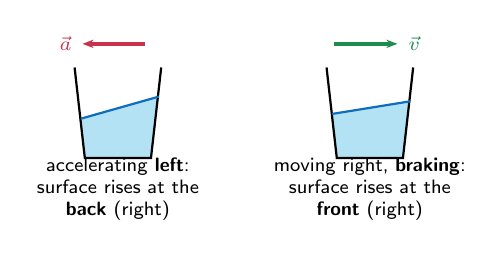
\begin{tikzpicture}[x=1cm, y=1cm, font=\scriptsize\sffamily]
  % glass 1: accelerating left
  \begin{scope}
    \fill[dsky!35] (-0.42,-0.6) -- (0.42,-0.6) -- (0.52,0.18) -- (-0.47,-0.10) -- cycle;
    \draw[thick] (-0.55,0.55) -- (-0.42,-0.6) -- (0.42,-0.6) -- (0.55,0.55);
    \draw[dblue, thick] (-0.47,-0.10) -- (0.52,0.18);
    \draw[-{Stealth[length=4pt]}, very thick, rosered] (0.35,0.85) -- (-0.45,0.85) node[left] {$\vec a$};
    \node[align=center] at (0,-1.0) {accelerating \textbf{left}:\\ surface rises at the\\ \textbf{back} (right)};
  \end{scope}
  % glass 2: braking while moving right (acceleration left too)
  \begin{scope}[xshift=3.2cm]
    \fill[dsky!35] (-0.42,-0.6) -- (0.42,-0.6) -- (0.51,0.12) -- (-0.48,-0.04) -- cycle;
    \draw[thick] (-0.55,0.55) -- (-0.42,-0.6) -- (0.42,-0.6) -- (0.55,0.55);
    \draw[dblue, thick] (-0.48,-0.04) -- (0.51,0.12);
    \draw[-{Stealth[length=4pt]}, very thick, dgreen] (-0.45,0.85) -- (0.35,0.85) node[right] {$\vec v$};
    \node[align=center] at (0,-1.0) {moving right, \textbf{braking}:\\ surface rises at the\\ \textbf{front} (right)};
  \end{scope}
\end{tikzpicture}
\figcap{The liquid surface tilts so it is \emph{higher on the side opposite the acceleration}.}
\end{center}
\begin{itemize}
\item A pendulum or hanging ball swings \emph{opposite} the acceleration (backward when speeding up).
\item A helium balloon does the reverse: it moves \emph{toward} the acceleration (the denser air sloshes back and pushes it forward).
\item Turning a corner: you feel pushed \emph{outward}; really, your body wants to keep going straight.
\item A cloth yanked quickly from under a glass leaves the glass behind (inertia).
\end{itemize}

\sub{B. Levers and torque}
\term{Torque} $=$ force $\times$ perpendicular distance from the pivot. A lever balances when clockwise torque $=$ counterclockwise torque: $F_1d_1=F_2d_2$.

{\footnotesize\renewcommand{\arraystretch}{1.1}
\begin{tabularx}{\linewidth}{@{}>{\leavevmode\bfseries\color{dnavy}}p{0.62in}>{\raggedright\arraybackslash}p{0.85in}L@{}}
\toprule
Class & In the middle & Examples\\\midrule
1st & Fulcrum & seesaw, crowbar, scissors, pliers, balance\\
2nd & Load & wheelbarrow, nutcracker, bottle opener, door\\
3rd & Effort & tweezers, broom, fishing rod, your forearm (biceps), tongs\\\bottomrule
\end{tabularx}}
\begin{itemize}
\item Mechanical advantage (MA) $=\dfrac{\text{effort arm}}{\text{load arm}}=\dfrac{\text{load}}{\text{effort}}$. A longer handle means less effort (wrench, door knob far from the hinges).
\item \term{Two people carrying a load on a pole}: the one \emph{closer} to the load carries more. A's share $=$ load $\times\frac{d_B}{L}$, where $d_B$ is the load's distance from B and $L$ is the pole's length.
\item 3rd-class levers have MA $<1$: they trade force for speed and range of motion.
\end{itemize}
\begin{dost}[Seesaw]
A 30-kg child sits 2 m from the pivot. Where must a 40-kg child sit to balance? $30(2)=40d\Rightarrow d=1.5$ m. The heavier child sits \emph{closer}.
\end{dost}

\sub{C. Gears, belts, and pulleys}
\begin{itemize}
\item \term{Meshed gears turn in opposite directions.} In a chain, gears 1, 3, 5, \ldots\ turn the same way as gear 1; gears 2, 4, \ldots\ turn the other way. Gears on the \emph{same shaft} turn together.
\item \term{Speed}: (teeth)$\times$(rpm) is the same for meshed gears. A small gear driven by a big one spins faster: $40$ teeth at 30 rpm drives 20 teeth at 60 rpm. Middle (idler) gears change direction, \emph{not} the final speed ratio.
\item Bigger driven gear $\Rightarrow$ slower but more torque (low gear on a bike for climbing).
\item Open belt: both wheels turn the same way. Crossed belt: opposite ways. Bicycle chain: same way.
\item \term{Fixed pulley}: changes the direction of the force only (MA $=1$). \term{Movable pulley}: MA $=2$. \term{Block and tackle}: MA $=$ number of rope segments holding up the movable block.
\item Work is conserved (ideal machine): if the effort is $\frac14$ of the load, you pull the rope \textbf{4 times} as far.
\end{itemize}

\sub{D. Other simple machines}
Inclined plane MA $=\dfrac{\text{length of slope}}{\text{height}}$ (a longer ramp is easier but longer) \textbullet\ wheel and axle MA $=\dfrac{R_\text{wheel}}{r_\text{axle}}$ (steering wheel, screwdriver) \textbullet\ wedge (axe, knife, zipper) \textbullet\ screw (an inclined plane wrapped around a cylinder; closer threads, larger MA). Efficiency $=\dfrac{\text{work out}}{\text{work in}}\times100\%<100\%$ because of friction.

\sub{E. Stability and center of gravity}
An object tips over when a vertical line through its \term{center of gravity} (CG) falls outside its base. \textbf{Lower CG + wider base = more stable} (racing cars, a bottle with sand at the bottom, standing with feet apart on a moving bus). Loading a truck high makes it easier to topple.

\sub{F. Fluids}
\begin{itemize}
\item \term{Pressure} $P=\dfrac FA$: sharp knives and nails (small $A$, large $P$); snowshoes and wide tires (large $A$, small $P$).
\item \term{Liquid pressure} $P=\rho gh$ grows with depth, not with the container's shape or width. A hole lower in a water bottle spurts out \textbf{faster and farther}. Dams are thicker at the bottom.
\item \term{Pascal's principle}: pressure applied to a confined fluid spreads equally. Hydraulic lift: $\dfrac{F_1}{A_1}=\dfrac{F_2}{A_2}$ (small push on a small piston lifts a car on a big one).
\item \term{Archimedes}: buoyant force $=$ weight of fluid displaced. An object floats if it is less dense than the fluid. Steel ships float because their hollow shape displaces a lot of water. Things float higher in seawater (denser) than in fresh water.
\item \term{Bernoulli}: faster-moving fluid has \textbf{lower pressure}. Airplane wings and kites get lift; strong winds lift roofs (fast air above, still air inside); two papers blown between move \emph{together}; a shower curtain is pulled inward.
\item \term{Continuity}: squeeze a hose nozzle (smaller area) and water comes out faster.
\end{itemize}

\sub{G. Heat in everyday things}
\begin{itemize}
\item \term{Conduction} (touch; metals conduct well, wood/plastic/air insulate) \textbullet\ \term{convection} (fluids circulate: boiling water, sea breeze, AC placed high, heater placed low) \textbullet\ \term{radiation} (no medium needed: sunlight, a campfire's warmth).
\item Dark, dull surfaces absorb and emit radiation best; shiny/white surfaces reflect (white roofs, emergency foil blankets).
\item \term{Thermal expansion}: gaps in bridges and railways; sagging power lines in summer; run hot water on a stuck metal lid. A \term{bimetallic strip} bends toward the metal that expands \emph{less} when heated (thermostats).
\end{itemize}

\sub{H. Springs, pendulums, and sound}
\begin{itemize}
\item \term{Hooke's law} $F=kx$: stretch is proportional to the load. Springs in \emph{series} stretch more (softer); springs side by side in \emph{parallel} stretch less (stiffer).
\item A pendulum's period depends only on its \textbf{length} (and $g$), not on its mass. Longer string $\Rightarrow$ slower swing.
\item Sound travels fastest in solids, slower in liquids, slowest in gases, and not at all in a vacuum. Light is far faster than sound, so you see lightning before you hear thunder.
\end{itemize}

\sub{I. Circuits and bulbs (a Primer favorite)}
\begin{itemize}
\item A bulb glows only in a \textbf{closed loop} through both battery terminals. A wire across a bulb (a \emph{short}) bypasses it: that bulb goes dark.
\item \term{Series}: one path, same current. Removing or burning out one bulb turns \emph{all} off. More bulbs in series $\Rightarrow$ all dimmer.
\item \term{Parallel}: separate paths, same voltage. Each bulb works on its own; adding bulbs does not dim the others (ideal battery) but drains the battery faster. Houses are wired in parallel.
\item Brightness follows power $P=I^2R$: more current through a bulb $\Rightarrow$ brighter.
\item Cells in series add voltage (two 1.5-V cells $=$ 3 V).
\item \term{Electromagnet} strength rises with more coil turns, more current, and an iron core. Like poles repel, unlike poles attract.
\end{itemize}
\begin{dost}[Mixed circuit]
Bulbs W and X are in parallel; that pair is in series with the parallel pair Y and Z. If Y burns out, the Y--Z group's resistance doubles, so the total current \textbf{drops}. W and X share less current: \textbf{dimmer}. Z now carries the whole (smaller) current, which is still more than its old half-share: \textbf{brighter}.
\end{dost}

% ============================================================ SPATIAL
\sect{2}{Spatial Reasoning}

You will see figure series, folded paper, cube nets, rotated solids, mirror images, and pieces to assemble. Work with \textbf{one distinctive feature at a time} instead of the whole picture.

\sub{A. Figure series}
Check each attribute separately: number of sides or elements (triangle, square, \textbf{pentagon}, hexagon, heptagon: $+1$ side), rotation per step (45$^\circ$, 90$^\circ$, clockwise or not), shading that alternates, an element moving around the corners, size growing or shrinking. A choice must satisfy \emph{every} rule at once.

\sub{B. Paper folding and hole punching}
\begin{itemize}
\item \term{Unfold in reverse order.} Each unfold \emph{mirrors} every hole across that fold line.
\item One punch through a sheet folded $n$ times (in half each time) makes $2^n$ holes.
\item \term{Folding without punching} (Primer type): a fold across a vertical line flips left--right; across a horizontal line flips top--bottom; a quadrant folded across \emph{both} lines ends up rotated 180$^\circ$. So a hole near the top-left of the bottom-right quarter lands at the \emph{bottom-right} of the folded square.
\end{itemize}

\sub{C. Cube nets and dice}
\begin{center}
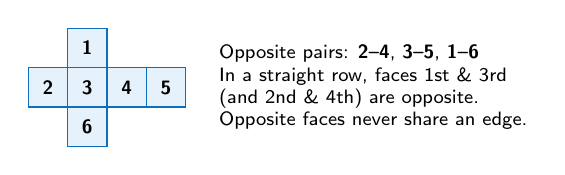
\begin{tikzpicture}[x=0.5cm, y=0.5cm, font=\scriptsize\sffamily\bfseries]
  \foreach \x/\y/\l in {1/1/1, 0/0/2, 1/0/3, 2/0/4, 3/0/5, 1/-1/6}{
    \draw[dblue, fill=dice] (\x,\y) rectangle ++(1,1);
    \node at (\x+0.5,\y+0.5) {\l};}
  \node[font=\scriptsize\sffamily, align=left, anchor=west] at (4.6,0.5)
    {Opposite pairs: \textbf{2--4}, \textbf{3--5}, \textbf{1--6}\\
     In a straight row, faces 1st \& 3rd\\ (and 2nd \& 4th) are opposite.\\
     Opposite faces never share an edge.};
\end{tikzpicture}
\figcap{A cross-shaped net of a cube.}
\end{center}
\begin{itemize}
\item A cube has 11 different nets. Faces that touch in the net (or meet at a corner when folded) are \emph{adjacent}, never opposite.
\item Standard dice: opposite faces add up to \textbf{7} (1--6, 2--5, 3--4), so you can never see 3 and 4 at the same time.
\item To check a folded-box choice: pick one face, find its true neighbors from the net, and see if the picture puts an opposite face beside it.
\end{itemize}

\sub{D. Rotation versus reflection}
A \term{rotation} keeps the figure's handedness; a \term{mirror image} reverses it. Rotate a \textsf{F} as much as you like and it never becomes \reflectbox{\textsf{F}}. To test a choice, trace a path around three distinctive features (clockwise order); in a true rotation that order is unchanged.
\begin{itemize}
\item \term{Vertical mirror} (to the left or right): left--right reversed; text reads backward, \reflectbox{AMBULANCE}. \term{Water/horizontal mirror}: top--bottom reversed.
\item Two reflections in a row restore the original (Primer-style: the spectrum seen in a mirror of a mirror reads normally).
\item \term{Clock in a mirror}: actual time $=$ 11:60 $-$ mirror time. Mirror 4:20 $\Rightarrow$ 7:40.
\item \term{Rotating a solid}: follow the odd feature (a notch, a slanted face) and its neighbors. Choices that move the feature to the wrong side are mirror images.
\end{itemize}

\sub{E. Assembling pieces and counting}
\begin{itemize}
\item Match unusual angles and edge lengths first; total area never changes; the number of pieces must match.
\item \term{Squares in an $n\times n$ grid}: $1^2+2^2+\cdots+n^2$ (3$\times$3 has 14; 4$\times$4 has 30).
\item \term{Painted cube} cut into $n^3$ unit cubes: 3 faces painted $=8$ (corners); 2 faces $=12(n-2)$; 1 face $=6(n-2)^2$; none $=(n-2)^3$.
\item Stacks of cubes: count column by column and include hidden cubes that must be there for support.
\item Euler: $V-E+F=2$ for any convex solid (cube: $8-12+6=2$).
\end{itemize}

\sub{F. Solids from flat shapes}
\textbf{Extrude} (slide) a shape to get a prism: circle $\to$ cylinder, triangle $\to$ triangular prism. \textbf{Spin} a shape about an axis: rectangle $\to$ cylinder, right triangle about a leg $\to$ cone, semicircle $\to$ sphere. Cross-sections: a cube can give a square, rectangle, triangle, or hexagon; a cone gives a circle, ellipse, parabola, hyperbola, or triangle.

% ============================================================ VERBAL
\sect{3}{Verbal Reasoning}

Analogies dominate the Primer's verbal items. Logic, series, and word roots fill the rest.

\sub{A. Solving analogies}
\begin{keybox}[Bridge sentence]
Turn the first pair into a precise sentence, then test each choice in the \emph{same} sentence. ``A \emph{lifebelt} keeps you safe in the \emph{sea}; a \emph{parachute} keeps you safe in the \emph{air}.'' If two choices fit, make the sentence stricter. Keep the \textbf{order} (A:B, not B:A) and the \textbf{part of speech} the same.
\end{keybox}
{\footnotesize\renewcommand{\arraystretch}{1.07}
\begin{tabularx}{\linewidth}{@{}>{\raggedright\arraybackslash\bfseries\color{dnavy}}p{1.02in}L@{}}
\toprule
Relationship & Example\\\midrule
Synonym / antonym & frankness : candor \textbullet\ anterior : posterior\\
Degree (milder $\to$ stronger) & warm : hot \textbullet\ affection : infatuation \textbullet\ timidity : cowardice \textbullet\ drizzle : downpour\\
Part : whole & petal : flower \textbullet\ chapter : book\\
Tool : worker & hammer : carpenter \textbullet\ brush : painter \textbullet\ scalpel : surgeon\\
Tool : function & scissors : cut \textbullet\ anemometer : wind speed\\
Worker : product & baker : bread \textbullet\ poet : poem\\
Member : group & fish : school \textbullet\ wolf : pack \textbullet\ lion : pride\\
Cause : effect & virus : infection \textbullet\ drought : famine\\
Lack of & drought : rain \textbullet\ darkness : light\\
Root : meaning & geo : earth \textbullet\ ferro : iron\\
Person : field/work & Newton : calculus \textbullet\ Copernicus : astronomy\\\bottomrule
\end{tabularx}}
\begin{caution}[Part of speech]
In the Primer item AFFECTION : INFATUATION, the answer is \emph{timidity : cowardice} (two nouns, the second an excessive, negative extreme of the first). \emph{large : gigantic} shows degree too, but they are adjectives, and the extreme is not a flaw.
\end{caution}

\sub{B. Word roots worth knowing}
{\footnotesize
\textbf{Elements and nature:} geo/terra earth \textbullet\ hydro/aqua water \textbullet\ pyro/igni fire \textbullet\ aero/pneumo air \textbullet\ litho/petro stone \textbullet\ helio/sol sun \textbullet\ luna/seleno moon \textbullet\ astro/stella star \textbullet\ ferro iron \textbullet\ cupr copper \textbullet\ argent silver \textbullet\ aur gold \textbullet\ plumb lead \textbullet\ photo light \textbullet\ thermo heat \textbullet\ chrono time \textbullet\ baro pressure \textbullet\ seismo earthquake \textbullet\ volcan fire/volcano.\par
\textbf{Life:} bio life \textbullet\ zoo animal \textbullet\ phyto plant \textbullet\ myco fungus \textbullet\ ichthy fish \textbullet\ ornith bird \textbullet\ entomo insect \textbullet\ herpeto reptile \textbullet\ anthropo human \textbullet\ cyte cell \textbullet\ derm skin \textbullet\ cardio heart \textbullet\ hemo blood \textbullet\ neuro nerve \textbullet\ osteo bone \textbullet\ gastro stomach \textbullet\ hepat liver \textbullet\ nephr/ren kidney \textbullet\ pulmo lung \textbullet\ ocul/ophthalm eye \textbullet\ oto ear \textbullet\ dent/odont tooth \textbullet\ cephal head \textbullet\ ped/pod foot \textbullet\ manu hand.\par
\textbf{Number and size:} mono/uni 1 \textbullet\ di/bi 2 \textbullet\ tri 3 \textbullet\ tetra/quad 4 \textbullet\ penta 5 \textbullet\ hexa 6 \textbullet\ hepta/sept 7 \textbullet\ octa 8 \textbullet\ nona 9 \textbullet\ deca 10 \textbullet\ centi 100 \textbullet\ milli 1000 \textbullet\ hemi/semi half \textbullet\ poly many \textbullet\ omni/pan all \textbullet\ micro small \textbullet\ macro/mega large.\par
\textbf{Position and relation:} sub/hypo under \textbullet\ super/hyper over \textbullet\ inter between \textbullet\ intra/endo within \textbullet\ exo/ecto outside \textbullet\ peri/circum around \textbullet\ trans across \textbullet\ tele far \textbullet\ anti/contra against \textbullet\ pre/ante before \textbullet\ post after \textbullet\ homo same \textbullet\ hetero different \textbullet\ iso equal \textbullet\ neo new \textbullet\ paleo old \textbullet\ auto self \textbullet\ ben good \textbullet\ mal bad \textbullet\ chloro green \textbullet\ erythro red \textbullet\ leuko white \textbullet\ melano black.\par
\textbf{Endings:} -logy study of \textbullet\ -meter measure \textbullet\ -scope view \textbullet\ -graph write/record \textbullet\ -phobia fear \textbullet\ -phile lover \textbullet\ -cide kill \textbullet\ -vore eat \textbullet\ -itis inflammation \textbullet\ -ectomy removal \textbullet\ -lysis splitting \textbullet\ -genesis origin \textbullet\ -troph nourishment.\par}

\sub{C. Scientists and their work}
{\footnotesize\renewcommand{\arraystretch}{1.04}
\begin{tabularx}{\linewidth}{@{}>{\raggedright\arraybackslash}p{1.45in}L@{}}
\toprule
Newton & laws of motion, gravitation, calculus\\
Copernicus & heliocentric (Sun-centered) model\\
Galileo & telescope astronomy, moons of Jupiter\\
Kepler & laws of planetary motion\\
Darwin / Mendel & natural selection / laws of inheritance\\
Lavoisier & conservation of mass\\
Dalton / Thomson / Rutherford / Bohr & atomic theory / electron / nucleus / energy levels\\
Mendeleev & periodic table\\
Hooke / Leeuwenhoek & named cells / first saw microorganisms\\
Schleiden, Schwann, Virchow & cell theory\\
Pasteur / Fleming / Jenner & germ theory / penicillin / smallpox vaccine\\
Watson \& Crick (with Franklin's data) & DNA double helix\\
Linnaeus & binomial nomenclature\\
Faraday / Ohm / Volta & induction / $V=IR$ / battery\\
Curie / Einstein / Hubble & radioactivity / relativity / expanding universe\\
Wegener / Hess & continental drift / seafloor spreading\\\bottomrule
\end{tabularx}}
\begin{keybox}[Filipino scientists]
\textbf{Fe del Mundo}: pediatrics, improved incubator \textbullet\ \textbf{Ramon Barba}: induced mango flowering with potassium nitrate \textbullet\ \textbf{Maria Orosa}: food technologist, banana ketchup \textbullet\ \textbf{Arturo Alcaraz}: father of Philippine volcanology, geothermal energy \textbullet\ \textbf{Angel Alcala}: marine biology, artificial reefs and marine sanctuaries \textbullet\ \textbf{Lourdes Cruz}: conotoxins from cone snails \textbullet\ \textbf{Eduardo Quisumbing}: Philippine medicinal plants and orchids \textbullet\ \textbf{Gregorio Zara}: two-way videophone \textbullet\ \textbf{Diosdado Banatao}: computer chip design \textbullet\ \textbf{Josette Biyo}: science teacher with a minor planet named after her.
\end{keybox}

\sub{D. Logic}
\begin{itemize}
\item \term{Syllogisms}: draw Venn circles; ``some'' means \emph{at least one}. Use only the given statements, not real-world facts.
  \begin{itemize}
  \item All A are B; all B are C $\Rightarrow$ all A are C.
  \item All A are B; no B is C $\Rightarrow$ no A is C.
  \item Some A are B; all B are C $\Rightarrow$ some A are C.
  \item All A are B; some B are C $\Rightarrow$ \textbf{nothing definite} about A and C.
  \item Some A are B; some B are C $\Rightarrow$ nothing definite.
  \end{itemize}
\item \term{Comparisons}: line people up on a number line. $M>O$ and $O<E$ tells you nothing about $M$ versus $E$.
\item \term{Conditionals}: ``If P then Q'' is equivalent to ``if not Q then not P.'' It does \emph{not} mean ``if Q then P.''
\item \term{Directions}: facing north, a right turn faces east, a left turn faces west, an about-turn faces south. Track the facing after every turn.
\end{itemize}

\sub{E. Series and codes}
\begin{itemize}
\item Letter positions: A1 E5 J10 O15 T20 Y25 (``EJOTY''). Reverse: Z$=$1st from the end.
\item Look for: constant differences, differences of differences ($2,6,12,20,30$: $+4,+6,+8,+10$), ratios, squares, cubes, primes, Fibonacci ($1,1,2,3,5,8,13,\ldots$), two series interleaved.
\item Famous ``hidden'' series: J, F, M, A, M, J, J, A, S, O, N, D (months), with 31, 28/29, 31, 30\ldots\ days; vowels A, E, I, O, U with positions 1, 5, 9, 15, 21.
\item \term{Codes}: compare letter positions of the word and its code (shift $+1$: CAT $\to$ DBU).
\end{itemize}

% ============================================================ LANGUAGE
\sect{4}{Language and Literature}

Grammar and syntax, vocabulary, functional English, and reading comprehension (the Primer's koala passage), plus basic literature.

\sub{A. Error spotting: the usual suspects}
\begin{itemize}
\item \term{Subject--verb agreement}: \emph{each, every, either, neither, everyone, nobody} are singular (``Each of the students \textbf{has}\ldots''). With \emph{or/nor}, agree with the nearer subject. \emph{As well as, along with, together with} don't change the subject. ``The number of'' is singular; ``a number of'' is plural. Collective nouns acting as one unit are singular (``The team \textbf{is} ready'').
\item \term{Pronoun case}: subjects use I/he/she/we/they; objects (after verbs and prepositions) use me/him/her/us/them: ``between you and \textbf{me}.'' Who (subject) vs.\ whom (object): answer with \emph{he} $\to$ who, \emph{him} $\to$ whom.
\item \term{Parallelism}: items joined by \emph{and/or} share one form. ``picked up the puppy, \textbf{straightened} her hat, and took it'' \yes; ``picked up\ldots, straightening\ldots, and took'' \no\ (the Primer's item).
\item \term{Modifiers}: put a phrase next to what it describes. ``Running to class, \emph{my bag} fell'' \no.
\item \term{Tense}: keep the sequence consistent; the earlier of two past actions takes \emph{had} + past participle. After an auxiliary (\emph{did, does, can, will}), use the base form: ``didn't \textbf{help}.''
\item \term{Adjective vs.\ adverb}: ``She sings \textbf{well}''; ``I feel \textbf{bad}'' (linking verb + adjective).
\item \term{Articles}: by sound, not spelling: \emph{an} hour, \emph{an} MRI, \emph{a} university, \emph{a} one-time offer.
\item \term{Comparisons}: \emph{fewer} (countable) vs.\ \emph{less} (uncountable); \emph{between} two vs.\ \emph{among} three or more; \emph{-er} for two, \emph{-est} for three or more; never ``more better.''
\item \term{Correlatives}: either\ldots\ \emph{or}, neither\ldots\ \emph{nor}, not only\ldots\ \emph{but also}, both\ldots\ \emph{and}.
\end{itemize}

\sub{B. Look-alike words}
{\footnotesize
\textbf{sometime} (an unspecified time: ``submit it sometime next month'') / \textbf{some time} (a period: ``it took some time'') / \textbf{sometimes} (occasionally) \textbullet\ \textbf{everyday} (adj., ordinary) / \textbf{every day} \textbullet\ \textbf{maybe} / \textbf{may be} \textbullet\ \textbf{already} / \textbf{all ready} \textbullet\ \textbf{altogether} (completely) / \textbf{all together} \textbullet\ \textbf{affect} (verb) / \textbf{effect} (noun; as a verb, ``to bring about'') \textbullet\ \textbf{its} / \textbf{it's} \textbullet\ \textbf{than} / \textbf{then} \textbullet\ \textbf{lose} / \textbf{loose} \textbullet\ \textbf{principal} / \textbf{principle} \textbullet\ \textbf{complement} / \textbf{compliment} \textbullet\ \textbf{stationary} / \textbf{stationery} \textbullet\ \textbf{advice} (n.) / \textbf{advise} (v.) \textbullet\ \textbf{adapt} / \textbf{adopt} \textbullet\ \textbf{beside} (next to) / \textbf{besides} (in addition) \textbullet\ \textbf{farther} (distance) / \textbf{further} (degree) \textbullet\ \textbf{imply} / \textbf{infer} \textbullet\ \textbf{eminent} (famous) / \textbf{imminent} (about to happen) \textbullet\ \textbf{emigrate} (leave) / \textbf{immigrate} (enter) \textbullet\ \textbf{lie} (recline: lie, lay, lain) / \textbf{lay} (put: lay, laid, laid) \textbullet\ \textbf{rise} (go up) / \textbf{raise} (lift something).\par}

\sub{C. Verb patterns and tags}
\begin{itemize}
\item Gerund after \emph{enjoy, avoid, finish, mind, consider, keep, suggest, practice}: ``Do you mind \textbf{opening}\ldots'' Infinitive after \emph{want, decide, hope, plan, agree, refuse}. ``Stop \textbf{to} buy'' (pause in order to) vs.\ ``stop \textbf{buying}'' (quit).
\item Conditionals: ``If I \textbf{were} you'' \textbullet\ ``If it rains, we \textbf{will} stay'' \textbullet\ ``If I \textbf{had known}, I \textbf{would have} come.''
\item Question tags flip the polarity: ``She is ready, \textbf{isn't she}?'' \textbullet\ ``I am late, \textbf{aren't I}?'' \textbullet\ ``Let's go, \textbf{shall we}?'' \textbullet\ ``Everyone came, \textbf{didn't they}?''
\item Reported speech shifts back: ``I \emph{am} tired'' $\to$ she said she \emph{was} tired; \emph{will} $\to$ \emph{would}; \emph{can} $\to$ \emph{could}.
\item Prepositions: different \emph{from}, interested \emph{in}, capable \emph{of}, good \emph{at}, consist \emph{of}, depend \emph{on}, comply \emph{with}, result \emph{in}, prefer X \emph{to} Y, arrive \emph{at} (a place) / \emph{in} (a city).
\end{itemize}

\sub{D. Functional English: the right response}
\begin{caution}[``Do you mind\ldots?'']
It literally asks ``Is it a problem for you?'' So the polite \emph{yes, I'll do it} is \textbf{``Not at all''} or ``No, go ahead.'' Answering ``Yes'' means you \emph{do} object. ``Would you mind if I sit here?'' $\to$ ``Not at all.''
\end{caution}
Thanks $\to$ ``You're welcome / It's my pleasure.'' \textbullet\ Apology $\to$ ``That's all right / No problem.'' \textbullet\ Offer (``Would you like some?'') $\to$ ``Yes, please'' or ``No, thank you.'' \textbullet\ ``How do you do?'' $\to$ ``How do you do?'' \textbullet\ ``May I\ldots?'' $\to$ ``Of course / Certainly.'' \textbullet\ Compliment $\to$ ``Thank you.''

\sub{E. Vocabulary}
Use \term{context clues}: a definition or restatement (\emph{that is, or}), a synonym nearby, a contrast (\emph{but, although, unlike}), examples (\emph{such as}), or the overall logic. Break unfamiliar words into roots (Section 3B). For ``which pair does NOT have the same meaning,'' look for the pair of opposites (\emph{shy -- effusive}).

{\footnotesize\renewcommand{\arraystretch}{1.02}
\begin{tabularx}{\linewidth}{@{}>{\leavevmode\bfseries}p{0.72in}L>{\leavevmode\bfseries}p{0.72in}L@{}}
\toprule
aloof & distant, cool & meticulous & very careful\\
ambiguous & unclear, two meanings & mitigate & lessen\\
amiable & friendly & mundane & ordinary\\
arduous & difficult, tiring & novel & new, original\\
benevolent & kind & obsolete & out of date\\
candid & frank, honest & placid & calm\\
conspicuous & easy to see & pragmatic & practical\\
corroborate & confirm & prudent & wise, careful\\
diligent & hardworking & reticent & reserved, quiet\\
effusive & gushing, expressive & resilient & recovers quickly\\
ephemeral & short-lived & scarce & few, rare\\
exacerbate & make worse & sporadic & now and then\\
frugal & thrifty & svelte & slim, graceful\\
futile & useless & tedious & boring, long\\
gregarious & sociable & tenacious & persistent\\
hinder & obstruct & terse & brief, curt\\
indolent & lazy & ubiquitous & everywhere\\
lethargic & sluggish & verbose & wordy\\
loquacious & talkative & vindicate & clear of blame\\
lucid & clear & zealous & eager, devoted\\\bottomrule
\end{tabularx}}

\sub{F. Idioms}
{\footnotesize piece of cake (very easy) \textbullet\ hit the books (study) \textbullet\ burn the midnight oil (work late) \textbullet\ break the ice (start a conversation) \textbullet\ under the weather (sick) \textbullet\ once in a blue moon (rarely) \textbullet\ cost an arm and a leg (very expensive) \textbullet\ beat around the bush (avoid the point) \textbullet\ spill the beans / let the cat out of the bag (reveal a secret) \textbullet\ bite the bullet (face something hard) \textbullet\ a blessing in disguise \textbullet\ call it a day (stop working) \textbullet\ hit the nail on the head (exactly right) \textbullet\ see eye to eye (agree) \textbullet\ on cloud nine (very happy) \textbullet\ add fuel to the fire (make worse) \textbullet\ the ball is in your court (your decision).\par}

\sub{G. Reading comprehension}
\begin{keybox}[Routine]
Read the questions first, then the passage. Answer only from the text: the Primer's koala passage says koalas are ``associated to wombats,'' so the answer is \emph{wombats and koala bears} even though no line says ``wombats are marsupials'' word for word. Restated words (``active only at night'' $=$ \emph{nocturnal}) are the most common right answers. Distrust extreme words (\emph{always, only, never, all}).
\end{keybox}
Question types: main idea / best title (covers the whole passage) \textbullet\ detail \textbullet\ vocabulary in context \textbullet\ inference (strongly implied) \textbullet\ author's purpose (inform, persuade, entertain, describe) \textbullet\ tone (objective, critical, nostalgic, humorous, optimistic, ironic) \textbullet\ sequence \textbullet\ cause and effect.

\sub{H. Literature essentials}
\begin{itemize}
\item \term{Plot}: exposition $\to$ rising action $\to$ \textbf{climax} (turning point) $\to$ falling action $\to$ resolution. \term{Conflict}: person vs.\ person, self, nature, society, technology, fate.
\item \term{Point of view}: first person (``I''), third-person limited, third-person omniscient (knows every mind). \term{Theme} is the message; \term{mood} is the reader's feeling; \term{tone} is the author's attitude.
\item \term{Devices}: foreshadowing, flashback, symbolism, imagery, allusion; irony---\emph{verbal} (saying the opposite), \emph{situational} (the opposite happens), \emph{dramatic} (the audience knows what a character doesn't).
\item \term{Poetry}: sonnet $=$ 14 lines (Shakespearean ABAB CDCD EFEF GG); haiku $=$ 5--7--5 syllables; iambic pentameter $=$ 10 syllables, da-DUM $\times5$; free verse has no fixed rhyme or meter; an elegy mourns; an ode praises; an epic tells of a hero.
\end{itemize}
{\footnotesize\renewcommand{\arraystretch}{1.04}
\begin{tabularx}{\linewidth}{@{}>{\leavevmode\bfseries\color{dnavy}}p{0.92in}L@{}}
\toprule
Simile & comparison with \emph{like/as}: ``as busy as a bee''\\
Metaphor & direct comparison: ``Time is a thief.''\\
Personification & human traits to things: ``the wind whispered''\\
Hyperbole & exaggeration: ``I've told you a million times''\\
Oxymoron & opposites side by side: ``deafening silence''\\
Paradox & seems contradictory but true: ``less is more''\\
Metonymy & a related thing stands for it: ``Malaca\~nang said\ldots''\\
Synecdoche & part for whole: ``all hands on deck''\\
Apostrophe & addressing the absent: ``O Death\ldots''\\
Onomatopoeia & sound words: \emph{buzz, tiktilaok}\\
Alliteration & repeated first sounds: ``Peter Piper picked''\\\bottomrule
\end{tabularx}}
\begin{keybox}[Philippine literature]
\textbf{Rizal}: \emph{Noli Me T\'angere} (1887), its sequel \emph{El Filibusterismo} (1891), ``Mi \'Ultimo Adi\'os,'' ``A la Juventud Filipina'' \textbullet\ \textbf{Balagtas}: \emph{Florante at Laura} \textbullet\ \textbf{Bonifacio}: ``Pag-ibig sa Tinubuang Lupa'' \textbullet\ \textbf{Paz M\'arquez-Benitez}: ``Dead Stars,'' a landmark early Filipino short story in English \textbullet\ \textbf{Nick Joaquin}: ``May Day Eve,'' \emph{The Woman Who Had Two Navels} \textbullet\ \textbf{Jos\'e Garc\'ia Villa}: the ``comma poems'' \textbullet\ \textbf{Carlos Bulosan}: \emph{America Is in the Heart} \textbullet\ \textbf{F.~Sionil Jos\'e}: the Rosales saga \textbullet\ \textbf{Manuel Arguilla}: ``How My Brother Leon Brought Home a Wife'' \textbullet\ \textbf{Lualhati Bautista}: \emph{Dekada '70} \textbullet\ \textbf{Severino Reyes}: \emph{Lola Basyang} tales. Epics: \emph{Biag ni Lam-ang} (Ilocano), \emph{Hudhud} (Ifugao), \emph{Hinilawod} (Panay), \emph{Darangen} (Maranao), \emph{Ibalon} (Bicol).
\end{keybox}
{\footnotesize\textbf{World literature quick list:} Homer (\emph{Iliad}, \emph{Odyssey}) \textbullet\ Sophocles (\emph{Oedipus Rex}) \textbullet\ Dante (\emph{Divine Comedy}) \textbullet\ Shakespeare (\emph{Romeo and Juliet}, \emph{Hamlet}, \emph{Macbeth}) \textbullet\ Cervantes (\emph{Don Quixote}) \textbullet\ Austen (\emph{Pride and Prejudice}, \emph{Emma}) \textbullet\ Dickens (\emph{Great Expectations}) \textbullet\ Mary Shelley (\emph{Frankenstein}) \textbullet\ Poe (``The Raven'') \textbullet\ Maupassant (``The Necklace'') \textbullet\ O.~Henry (``The Gift of the Magi'') \textbullet\ Orwell (\emph{Animal Farm}, \emph{1984}) \textbullet\ Harper Lee (\emph{To Kill a Mockingbird}) \textbullet\ Hemingway (\emph{The Old Man and the Sea}) \textbullet\ Achebe (\emph{Things Fall Apart}) \textbullet\ Saint-Exup\'ery (\emph{The Little Prince}) \textbullet\ Machiavelli (\emph{The Prince}) \textbullet\ Margery Williams (\emph{The Velveteen Rabbit}).\par}

% ============================================================ BIOLOGY
\sect{5}{Biology}

\sub{A. Cells}
{\footnotesize\renewcommand{\arraystretch}{1.04}
\begin{tabularx}{\linewidth}{@{}>{\leavevmode\bfseries\color{dnavy}}p{0.95in}L@{}}
\toprule
Nucleus & holds DNA; controls the cell\\
Ribosome & makes proteins (free, or on rough ER)\\
Rough / smooth ER & protein transport / lipid synthesis, detox\\
Golgi apparatus & modifies, packages, ships proteins\\
Mitochondrion & cellular respiration; makes ATP (``powerhouse'')\\
Chloroplast & photosynthesis (plants, algae)\\
Lysosome & digestive enzymes (mostly animal cells)\\
Vacuole & storage; one large central vacuole in plants\\
Cell membrane & phospholipid bilayer; selectively permeable\\
Cell wall & cellulose (plants), chitin (fungi)\\
Cilia / flagella & movement; powered by the motor protein dynein\\
Centrioles & help organize cell division (animal cells)\\\bottomrule
\end{tabularx}}
\begin{itemize}
\item \term{Prokaryotes} (bacteria, archaea): no nucleus, no membrane-bound organelles, have ribosomes. \term{Eukaryotes}: nucleus and organelles.
\item Plant cells have a cell wall, chloroplasts, and a large vacuole; animal cells have centrioles and lysosomes. \term{Cell theory}: all living things are made of cells; the cell is the basic unit of life; cells come from pre-existing cells.
\end{itemize}

\sub{B. Moving things across membranes}
\begin{itemize}
\item \term{Diffusion}: high $\to$ low concentration, no energy. \term{Osmosis}: diffusion of \emph{water} across a membrane, toward the side with more solute. \term{Active transport}: low $\to$ high, uses ATP (sodium--potassium pump).
\item In a \term{hypotonic} solution (e.g., distilled water) water rushes in: animal cells swell and may burst (lysis); plant cells become firm (turgid). In a \term{hypertonic} solution (e.g., salty water) water leaves: animal cells shrivel (crenation); plant cells undergo plasmolysis. \term{Isotonic}: no net change.
\end{itemize}

\sub{C. Biomolecules and enzymes}
\textbf{Carbohydrates}: glucose; sucrose $=$ glucose $+$ fructose; lactose $=$ glucose $+$ galactose; starch (plant storage), glycogen (animal storage), cellulose (plant cell walls). \textbf{Lipids}: fats, oils, phospholipids, steroids. \textbf{Proteins}: amino acids joined by peptide bonds. \textbf{Nucleic acids}: DNA and RNA, made of nucleotides. \textbf{Enzymes} are proteins that speed up reactions by lowering activation energy; they are specific (lock and key) and are denatured by extreme heat or pH. Food tests: iodine (starch $\to$ blue-black), Benedict's (simple sugars $\to$ brick red on heating), Biuret (protein $\to$ violet).

\sub{D. Energy in cells}
\begin{formbox}[Two key equations]
Photosynthesis: $6\chem{CO_2}+6\chem{H_2O}\xrightarrow{\text{light}}\chem{C_6H_{12}O_6}+6\chem{O_2}$\\
Respiration: $\chem{C_6H_{12}O_6}+6\chem{O_2}\to6\chem{CO_2}+6\chem{H_2O}+\text{ATP}$
\end{formbox}
\begin{itemize}
\item Photosynthesis: \emph{light reactions} in the thylakoids split water (releasing O$_2$) and make ATP and NADPH; the \emph{Calvin cycle} in the stroma fixes CO$_2$ into sugar.
\item Respiration: \textbf{glycolysis} (cytoplasm, 2 ATP net) $\to$ \textbf{Krebs cycle} (mitochondrial matrix, 2 ATP) $\to$ \textbf{electron transport chain} (inner membrane, most ATP). Total $\approx36$--38 ATP per glucose.
\item Without oxygen: lactic acid fermentation (tired muscles) or alcoholic fermentation (yeast: ethanol $+$ CO$_2$, which raises bread).
\end{itemize}

\sub{E. Cell division}
{\footnotesize\renewcommand{\arraystretch}{1.06}
\begin{tabularx}{\linewidth}{@{}>{\leavevmode\bfseries\color{dnavy}}p{0.75in}LL@{}}
\toprule
 & Mitosis & Meiosis\\\midrule
Purpose & growth, repair, asexual reproduction & makes gametes (sperm, egg)\\
Divisions & 1 & 2\\
Products & 2 identical diploid ($2n$) cells & 4 different haploid ($n$) cells\\
Human example & 46 $\to$ 46 & 46 $\to$ 23\\
Variation & none & crossing over (prophase I), independent assortment\\\bottomrule
\end{tabularx}}
Stages: interphase (DNA copied in the S phase) $\to$ \textbf{P}rophase $\to$ \textbf{M}etaphase (chromosomes line up at the middle) $\to$ \textbf{A}naphase (pulled apart) $\to$ \textbf{T}elophase $\to$ cytokinesis. If cells divide every 18 h, then in 48 h a cell completes 2 divisions: $1\to4$ cells.

\sub{F. Genetics}
\begin{itemize}
\item \term{Mendel}: law of \emph{segregation} (allele pairs separate into gametes), \emph{independent assortment}, \emph{dominance}. Genotype $=$ alleles (Tt); phenotype $=$ trait (tall).
\item $Tt\times Tt$: genotypes 1 TT : 2 Tt : 1 tt; phenotypes \textbf{3 : 1}. $Tt\times tt$ (test cross): 1 : 1. Dihybrid $AaBb\times AaBb$: \textbf{9 : 3 : 3 : 1}.
\item \term{Incomplete dominance}: blend (red $\times$ white $\to$ pink; pink $\times$ pink $\to$ 1 red : 2 pink : 1 white). \term{Codominance}: both show (roan cattle; AB blood).
\item \term{ABO blood}: A $=I^AI^A$ or $I^Ai$; B $=I^BI^B$ or $I^Bi$; AB $=I^AI^B$; O $=ii$. Two type-O parents can only have type-O children.
\item \term{X-linked recessive} (hemophilia, red--green color blindness): far more common in males (one X). An affected father passes the allele to \emph{all daughters} (carriers) and to \emph{no sons}. A carrier mother gives each son a $\frac12$ chance of being affected.
\item \term{Pedigrees}: squares $=$ males, circles $=$ females, shaded $=$ affected. Skips a generation $\to$ recessive. Mostly males, passed through carrier mothers $\to$ X-linked recessive. Affected father with affected son $\to$ not X-linked.
\item Multiply independent probabilities: $P(\text{son})\times P(\text{albino})\times\cdots$
\end{itemize}

\sub{G. DNA, RNA, and proteins}
\begin{itemize}
\item DNA: double helix, deoxyribose, bases \textbf{A--T} and \textbf{G--C}. RNA: single strand, ribose, \textbf{U} replaces T. DNA replication is semi-conservative.
\item \term{Central dogma}: DNA $\xrightarrow{\text{transcription (nucleus)}}$ mRNA $\xrightarrow{\text{translation (ribosome)}}$ protein. Codons are 3 bases; AUG $=$ start (methionine); UAA, UAG, UGA $=$ stop. tRNA carries amino acids and has the anticodon.
\item Template DNA 3$'$-TAC GGA-5$'$ $\to$ mRNA 5$'$-AUG CCU-3$'$ (pair each base; use U for A).
\item Mutations: substitution (may be silent), insertion or deletion (frameshift, usually severe). Chromosome errors: Down syndrome (trisomy 21), Turner (XO), Klinefelter (XXY).
\item Biotechnology: PCR \emph{amplifies} (copies) DNA; gel electrophoresis separates DNA by size (small pieces travel farthest); recombinant DNA and GMOs (Golden Rice makes beta-carotene, Bt crops resist insects).
\end{itemize}

\sub{H. Evolution and classification}
\begin{itemize}
\item \term{Natural selection} (Darwin): variation $+$ overproduction $+$ competition $\Rightarrow$ the best-adapted survive and reproduce more. Lamarck's ``use and disuse'' is rejected.
\item Evidence: fossils; \term{homologous} structures (same bones, different uses: human arm, bat wing, whale flipper $\Rightarrow$ common ancestor); \term{analogous} structures (same use, different origin: bird wing vs.\ insect wing); \term{vestigial} structures (appendix, tailbone); similar embryos; DNA similarity.
\item On a cladogram or tree, the latest branching point marks the most recently diverged groups.
\item Taxonomy: Domain, Kingdom, Phylum, Class, Order, Family, Genus, Species (``Dear King Philip Came Over For Good Soup''). Scientific names: \emph{Homo sapiens}, \emph{Pithecophaga jefferyi} (Philippine eagle).
\item Three domains: Bacteria, Archaea, Eukarya (protists, fungi, plants, animals).
\item Animal phyla: sponges (Porifera); jellyfish, corals (Cnidaria); flatworms; roundworms; segmented worms (Annelida); snails, clams, squid (Mollusca); insects (6 legs), spiders (8 legs), crustaceans (Arthropoda); sea stars, sea urchins (Echinodermata); Chordata (tunicates and vertebrates: fish, amphibians, reptiles, birds, mammals).
\item Plants: mosses (no vascular tissue) $\to$ ferns (vascular, spores) $\to$ gymnosperms (naked seeds, conifers) $\to$ angiosperms (flowers, seeds in fruit). Monocots (1 cotyledon, parallel veins, flower parts in 3s: rice, corn) vs.\ dicots (2 cotyledons, net veins, parts in 4s or 5s: mongo, mango).
\end{itemize}

\sub{I. Plants}
Xylem carries water up from the roots; phloem carries sugar. Stomata (opened and closed by guard cells) let in CO$_2$ and lose water (transpiration). Flower: stamen $=$ anther $+$ filament (male); pistil $=$ stigma $+$ style $+$ ovary (female); the ovary becomes the fruit, ovules become seeds. Tropisms: phototropism (light), gravitropism, thigmotropism (touch). Hormones: auxin (growth toward light), gibberellin (stem growth), ethylene (ripening; why calcium carbide or a ripe banana speeds ripening), abscisic acid (closes stomata).

\sub{J. Human body systems}
{\footnotesize\renewcommand{\arraystretch}{1.04}
\begin{tabularx}{\linewidth}{@{}>{\leavevmode\bfseries\color{dnavy}}p{0.78in}L@{}}
\toprule
Digestive & mouth (amylase) $\to$ esophagus $\to$ stomach (HCl, pepsin) $\to$ \textbf{small intestine} (most digestion and absorption; villi) $\to$ large intestine (absorbs water). Liver makes bile (emulsifies fat); pancreas makes enzymes and insulin.\\
Respiratory & nose $\to$ pharynx $\to$ larynx $\to$ trachea $\to$ bronchi $\to$ bronchioles $\to$ \textbf{alveoli} (gas exchange). The diaphragm contracts to inhale.\\
Circulatory & 4-chambered heart; right side pumps blood to the lungs, left ventricle (thickest wall) to the body. Arteries carry blood \emph{away} from the heart (the pulmonary artery carries deoxygenated blood!), veins \emph{toward}. RBCs carry O$_2$ (hemoglobin), WBCs fight infection, platelets clot.\\
Excretory & kidney (nephrons filter blood) $\to$ renal pelvis $\to$ \textbf{ureter} $\to$ urinary \textbf{bladder} $\to$ \textbf{urethra}.\\
Nervous & neuron: dendrite $\to$ cell body $\to$ axon. Cerebrum (thinking, senses), cerebellum (balance, coordination), medulla (breathing, heartbeat). Reflexes pass through the spinal cord.\\
Endocrine & pituitary (``master gland''), thyroid (metabolism), pancreas (insulin lowers, glucagon raises blood sugar), adrenal (adrenaline), ovaries and testes.\\
Others & skeletal (206 adult bones), muscular (skeletal $=$ voluntary; smooth and cardiac $=$ involuntary), immune (antibodies; vaccines train memory cells), integumentary (skin).\\\bottomrule
\end{tabularx}}
\begin{keybox}[Hearing pathway]
Outer ear (pinna, ear canal) $\to$ \textbf{eardrum} (tympanic membrane) $\to$ hammer, anvil, stirrup (malleus, incus, stapes) $\to$ \textbf{oval window} $\to$ fluid of the \textbf{cochlea} (basilar membrane, hair cells) $\to$ auditory nerve. The round window relieves pressure. The \textbf{Eustachian tube} only equalizes air pressure; sound does not travel through it.
\end{keybox}

\sub{K. Ecology}
\begin{itemize}
\item Levels: organism $\to$ population $\to$ community $\to$ ecosystem $\to$ biome $\to$ biosphere. Producers (plants, algae, phytoplankton) $\to$ primary consumers (herbivores) $\to$ secondary $\to$ tertiary consumers; decomposers (bacteria, fungi) recycle nutrients. A fruit and the tree it grows on are both at the producer level; the Sun is not an organism.
\item \term{10\% rule}: only about 10\% of the energy passes to the next level. 10{,}000 kJ in grass $\to$ 1{,}000 $\to$ 100 $\to$ 10 kJ. Top consumers get the least energy; toxins like mercury and DDT build up most in them (\emph{biomagnification}).
\item \term{Symbiosis}: mutualism ($+/+$: legumes and \emph{Rhizobium}, coral and algae, clownfish and anemone, lichens); commensalism ($+/0$: orchid on a tree, barnacles on a whale); parasitism ($+/-$: tapeworm, lice); also predation and competition.
\item \term{Nitrogen cycle}: N$_2$ fixed by bacteria in legume root nodules (and lightning) $\to$ ammonia $\to$ nitrites $\to$ nitrates (taken up by plants) $\to$ back to N$_2$ by denitrifying bacteria. Rotating crops with legumes (mongo, peanuts, soybeans) restores soil nitrogen; more legume seasons $=$ more nitrogen.
\item \term{Carbon cycle}: photosynthesis removes CO$_2$; respiration, decomposition, and burning fuels return it.
\item Population density $=\dfrac{\text{number of individuals}}{\text{area occupied}}$. Exponential (J) growth vs.\ logistic (S) growth that levels off at the \emph{carrying capacity}. Age pyramids: wide base $=$ growing; narrow base $=$ shrinking.
\item Succession: \emph{primary} on bare rock (lichens and mosses first); \emph{secondary} after a fire or on abandoned farmland (soil remains).
\item The Philippines is \emph{megadiverse} with many endemic species: Philippine eagle, tarsier, tamaraw (Mindoro), Philippine cockatoo.
\end{itemize}

% ============================================================ CHEMISTRY
\sect{6}{Chemistry}

\sub{A. Matter and its changes}
\begin{itemize}
\item Phase changes: melting, freezing, evaporation/boiling, condensation, \textbf{sublimation} (solid $\to$ gas: dry ice, mothballs), deposition (gas $\to$ solid). Boiling water breaks the attractions \emph{between} molecules, not the O--H bonds inside them (it stays H$_2$O).
\item \term{Physical change}: same substance (cutting, dissolving, melting). \term{Chemical change}: new substance; signs are gas bubbles, a precipitate, a color change, heat or light, a new odor (rusting, burning, cooking, rotting).
\item \term{Pure substances}: elements and compounds. \term{Mixtures}: homogeneous (solutions: salt water, air, brass) or heterogeneous (suspensions settle; colloids such as milk and fog scatter light, the Tyndall effect).
\item Separation: filtration (insoluble solid), evaporation (dissolved solid), distillation and fractional distillation (different boiling points), \textbf{chromatography} (components travel at different rates; identical spot patterns $=$ same ink), decantation, centrifuge, magnet.
\end{itemize}

\sub{B. Atoms}
\begin{itemize}
\item Atomic number $Z=$ protons. Mass number $A=$ protons $+$ neutrons. In a neutral atom, electrons $=$ protons. $^{56}_{26}$Fe has 26 p, 30 n, 26 e. $^{35}$Cl$^-$ has 17 p, 18 n, \textbf{18} e.
\item \term{Isotopes}: same protons, different neutrons (C-12, C-14). \term{Ions}: cations lost electrons ($+$), anions gained electrons ($-$).
\item Models: Dalton (solid sphere) $\to$ Thomson (plum pudding; discovered the electron) $\to$ Rutherford (gold foil: tiny dense positive nucleus) $\to$ Bohr (fixed energy levels) $\to$ quantum model (orbitals).
\item Electron configuration order: 1s 2s 2p 3s 3p \textbf{4s 3d} 4p 5s 4d\ldots; s holds 2, p 6, d 10, f 14. Na: 1s$^2$2s$^2$2p$^6$3s$^1$.
\end{itemize}

\sub{C. The periodic table}
\begin{itemize}
\item Groups (columns) share valence electrons and properties; periods (rows) share the number of shells. For main groups, valence electrons $=$ last digit of the group number.
\item Group 1 alkali metals ($+1$, very reactive with water); group 2 alkaline earth ($+2$); groups 3--12 transition metals; group 17 halogens ($-1$); group 18 noble gases (full shells, unreactive). Metalloids along the staircase: B, Si, Ge, As, Sb, Te.
\end{itemize}
\begin{formbox}[Periodic trends]
Across a period ($\rightarrow$): atomic radius \textbf{decreases}; ionization energy and electronegativity \textbf{increase}.\\
Down a group ($\downarrow$): radius \textbf{increases}; ionization energy and electronegativity \textbf{decrease}.\\
Fluorine is the most electronegative element; francium/cesium the most metallic. Cations are smaller than their atoms; anions are larger.
\end{formbox}

\sub{D. Bonding and shapes}
\begin{itemize}
\item \term{Ionic}: metal $+$ nonmetal, electrons transferred; high melting points; conduct when melted or dissolved. \term{Covalent}: nonmetals share electrons (polar if electronegativities differ). \term{Metallic}: a ``sea'' of electrons (conductive, malleable).
\item \term{Writing ionic formulas}: cross the charges and reduce. Al$^{3+}$ $+$ O$^{2-}$ $\to$ Al$_2$O$_3$; Ca$^{2+}$ $+$ Cl$^-$ $\to$ CaCl$_2$; Al$^{3+}$ $+$ SO$_4^{2-}$ $\to$ Al$_2$(SO$_4$)$_3$; a $2+$ metal with a $4-$ ion gives M$_2$X (Primer-style: ``M$_2$X needs X$^{4-}$'').
\end{itemize}
{\footnotesize\renewcommand{\arraystretch}{1.05}
\begin{tabularx}{\linewidth}{@{}>{\raggedright\arraybackslash}p{0.85in}>{\raggedright\arraybackslash}p{1.05in}L@{}}
\toprule
\textbf{Bonding / lone pairs} & \textbf{Shape (angle)} & \textbf{Example}\\\midrule
2 / 0 & linear (180$^\circ$) & CO$_2$, BeCl$_2$\\
3 / 0 & trigonal planar (120$^\circ$) & BF$_3$\\
4 / 0 & tetrahedral (109.5$^\circ$) & CH$_4$\\
3 / 1 & \textbf{trigonal pyramidal} (107$^\circ$) & NH$_3$ (central atom with 5 valence e$^-$)\\
2 / 2 & bent (104.5$^\circ$) & H$_2$O\\\bottomrule
\end{tabularx}}
\begin{itemize}
\item Symmetric molecules are nonpolar even with polar bonds (CO$_2$, CH$_4$); H$_2$O and NH$_3$ are polar. ``Like dissolves like.''
\item Intermolecular forces: London dispersion $<$ dipole--dipole $<$ \textbf{hydrogen bonding} (H on N, O, or F). Stronger forces $\Rightarrow$ higher boiling point. Water's hydrogen bonds explain its high boiling point and surface tension.
\item \term{Soap and detergent}: a polar/ionic \textbf{head} (attracted to water) and a long nonpolar \textbf{tail} (dissolves in grease). Tails point \emph{into} the grease, heads face the water (a micelle).
\end{itemize}

\sub{E. Names and formulas}
{\footnotesize Polyatomic ions: NH$_4^+$ ammonium \textbullet\ OH$^-$ hydroxide \textbullet\ NO$_3^-$ nitrate \textbullet\ NO$_2^-$ nitrite \textbullet\ SO$_4^{2-}$ sulfate \textbullet\ SO$_3^{2-}$ sulfite \textbullet\ CO$_3^{2-}$ carbonate \textbullet\ HCO$_3^-$ bicarbonate \textbullet\ PO$_4^{3-}$ phosphate \textbullet\ CH$_3$COO$^-$ acetate \textbullet\ MnO$_4^-$ permanganate. Naming: FeCl$_3$ iron(III) chloride; N$_2$O$_4$ dinitrogen tetroxide; CO carbon monoxide. Common names: NaCl table salt \textbullet\ NaHCO$_3$ baking soda \textbullet\ NaOH lye \textbullet\ CaCO$_3$ limestone, chalk, shells \textbullet\ CaO quicklime \textbullet\ HCl muriatic acid \textbullet\ CH$_3$COOH acetic acid (vinegar) \textbullet\ C$_2$H$_5$OH ethanol \textbullet\ NaClO bleach \textbullet\ propane/butane (LPG) \textbullet\ CH$_4$ methane \textbullet\ solid CO$_2$ dry ice \textbullet\ Mg(OH)$_2$ milk of magnesia.\par}

\sub{F. Moles and stoichiometry}
\begin{formbox}
$n=\dfrac{\text{mass}}{\text{molar mass}}$ \textbullet\ 1 mol $=6.02\times10^{23}$ particles \textbullet\ 1 mol of gas at STP $=22.4$ L\\
Atomic masses: H 1, C 12, N 14, O 16, Na 23, Mg 24, Al 27, S 32, Cl 35.5, K 39, Ca 40, Fe 56, Cu 63.5
\end{formbox}
\begin{itemize}
\item Molar mass of CO$_2$ $=12+2(16)=44$ g/mol, so 0.5 mol $=22$ g. Percent of O in H$_2$O $=\frac{16}{18}\approx89\%$.
\item Balance equations by counting atoms (mass is conserved): $2\chem{H_2}+\chem{O_2}\to2\chem{H_2O}$. Mole ratios come from the coefficients. The \term{limiting reactant} runs out first and decides the yield.
\end{itemize}

\sub{G. Reactions}
\begin{itemize}
\item Synthesis (A $+$ B $\to$ AB) \textbullet\ decomposition (AB $\to$ A $+$ B) \textbullet\ single replacement (A $+$ BC $\to$ AC $+$ B) \textbullet\ double replacement (forms a precipitate, gas, or water) \textbullet\ combustion (fuel $+$ O$_2$ $\to$ CO$_2$ $+$ H$_2$O) \textbullet\ neutralization (acid $+$ base $\to$ salt $+$ water).
\item \term{Activity series}: K $>$ Na $>$ Ca $>$ Mg $>$ Al $>$ Zn $>$ Fe $>$ Ni $>$ Sn $>$ Pb $>$ (H) $>$ Cu $>$ Ag $>$ Au. A metal replaces only metals \emph{below} it: Zn $+$ CuSO$_4$ works; Cu $+$ ZnSO$_4$ does not. Metals above H release H$_2$ from acids.
\item \term{Redox}: OIL RIG (Oxidation Is Loss, Reduction Is Gain of electrons).
\item \term{Rates} increase with temperature, concentration, surface area (powder $>$ lump), and a catalyst (lowers activation energy, not used up). \term{Le Ch\^atelier}: a system at equilibrium shifts to undo a change.
\item \term{Exothermic} releases heat (combustion, freezing, condensation, neutralization). \term{Endothermic} absorbs heat (melting, evaporation, photosynthesis, instant cold packs). $q=mc\Delta T$ ($c_\text{water}=4.18$ J/g$\cdot^\circ$C).
\end{itemize}

\sub{H. Gas laws}
\begin{formbox}[Always use kelvins: K $=$ $^\circ$C $+$ 273]
Boyle $P_1V_1=P_2V_2$ \textbullet\ Charles $\dfrac{V_1}{T_1}=\dfrac{V_2}{T_2}$ \textbullet\ Gay-Lussac $\dfrac{P_1}{T_1}=\dfrac{P_2}{T_2}$ \textbullet\ Avogadro $\dfrac{V_1}{n_1}=\dfrac{V_2}{n_2}$\\
Combined $\dfrac{P_1V_1}{T_1}=\dfrac{P_2V_2}{T_2}$ \textbullet\ Ideal gas $PV=nRT$, $R=0.0821$ L$\cdot$atm/(mol$\cdot$K) \textbullet\ STP: 0$^\circ$C, 1 atm
\end{formbox}
\begin{dost}[Primer Science item 2]
25.0 L, 1.00 atm, 35$^\circ$C (308 K) $\to$ 20.0 L, 2.00 atm. $T_2=308\times\frac{(2.00)(20.0)}{(1.00)(25.0)}=308\times1.6=492.8$ K $=$ \textbf{220$^\circ$C}. The choice ``493'' is the kelvin value: a trap.
\end{dost}
Heating a gas in a sealed rigid cylinder raises its pressure, molecular speed, and kinetic energy, but the average distance between molecules stays the same (volume is fixed).

\sub{I. Solutions, acids, and bases}
\begin{itemize}
\item Molarity $M=\dfrac{\text{mol solute}}{\text{L solution}}$; dilution $M_1V_1=M_2V_2$. Most solids dissolve better when hot; gases dissolve \emph{less} when hot and \emph{more} under pressure (soda fizzes when opened). Salt lowers the freezing point and raises the boiling point of water.
\item $\text{pH}=-\log[\text{H}^+]$: below 7 acidic, 7 neutral, above 7 basic. Each pH unit is a \textbf{10-fold} change: pH 3 has 100 times the [H$^+$] of pH 5. pH $+$ pOH $=14$.
\item Acids taste sour, turn blue litmus red, react with active metals; bases taste bitter, feel slippery, turn red litmus blue. Phenolphthalein: colorless in acid, pink in base.
\item \term{Choosing an indicator}: pick one whose color-change range covers the pH you are checking (methyl orange about 3--4.4, methyl red about 4.4--6.2, bromothymol blue about 6--7.6, phenolphthalein about 8.2--10).
\item Acid rain (pH below 5.6) comes from SO$_2$ and nitrogen oxides. Strong acids: HCl, HNO$_3$, H$_2$SO$_4$. Household bases: ammonia, soap, baking soda, antacids.
\end{itemize}

\sub{J. Nuclear and organic chemistry}
\begin{itemize}
\item Alpha ($^4_2$He; stopped by paper) \textbullet\ beta (electron; stopped by aluminum) \textbullet\ gamma (energy; needs lead or concrete). Fission splits heavy nuclei (nuclear plants); fusion joins light nuclei (the Sun).
\item \term{Half-life}: amount left $=$ start $\times\left(\frac12\right)^{t/T}$. 80 g with $T=5$ days $\to$ 10 g after 15 days.
\item Hydrocarbons: alkanes (single bonds, C$_n$H$_{2n+2}$, -ane), alkenes (double, -ene), alkynes (triple, -yne). Prefixes: meth 1, eth 2, prop 3, but 4, pent 5, hex 6, hept 7, oct 8. Functional groups: alcohol $-$OH, carboxylic acid $-$COOH, ester (fruity smells), amine $-$NH$_2$.
\item Lab basics: read a graduated cylinder at the \emph{bottom of the meniscus}, eye level; always add acid to water; point test tubes away from people.
\end{itemize}

% ============================================================ EARTH SCIENCE
\sect{7}{Earth Science}

\sub{A. Inside the Earth}
Crust (oceanic: thin, dense basalt; continental: thick, lighter granite) $\to$ mantle (lithosphere $=$ crust $+$ rigid upper mantle; asthenosphere is soft and flowing) $\to$ \textbf{liquid outer core} (iron--nickel; makes Earth's magnetic field) $\to$ solid inner core.
\begin{itemize}
\item \term{P waves}: fastest, push--pull, travel through solids and liquids. \term{S waves}: slower, side-to-side, \textbf{solids only}; the S-wave shadow zone shows the outer core is liquid. \term{Surface waves}: slowest, most damaging.
\end{itemize}

\sub{B. Plate tectonics}
\begin{itemize}
\item \term{Continental drift} (Wegener): Pangaea; evidence from matching coastlines, fossils (\emph{Mesosaurus}, \emph{Glossopteris}), rock layers, and ancient climates. \term{Seafloor spreading} (Hess): new crust forms at mid-ocean ridges; rocks get older away from the ridge. Mantle convection moves the plates.
\item \term{Divergent}: plates separate (mid-Atlantic ridge, rift valleys). \term{Convergent}: oceanic under continental $\to$ trench $+$ volcanic mountains; oceanic under oceanic $\to$ trench $+$ volcanic island arc (the Philippines, Japan); continent--continent $\to$ folded mountains (Himalayas). \term{Transform}: plates slide past each other (earthquakes, no volcanoes).
\item \term{The Philippines} sits on the \emph{Ring of Fire} between the Philippine Sea Plate and the Eurasian Plate. The Philippine Trench (east) and Manila Trench (west) are subduction zones. The Philippine Fault Zone runs from Luzon to Mindanao; the West Valley Fault crosses Metro Manila.
\end{itemize}

\sub{C. Earthquakes}
\begin{itemize}
\item \term{Focus} (hypocenter): where the rupture starts underground. \term{Epicenter}: the point on the surface directly above it. Locating an epicenter needs at least \textbf{three} stations (triangulation using the S--P time lag).
\item \term{Magnitude}: energy released (one value per quake; each whole number $\approx$ 32 times more energy). \term{Intensity}: effects at a place (varies by location; PHIVOLCS Earthquake Intensity Scale, I to X).
\item Faults: normal (pulled apart; hanging wall drops), reverse/thrust (pushed together; hanging wall rises), strike-slip (sideways).
\item Hazards: ground shaking, liquefaction, landslides, tsunamis (warning sign: the sea suddenly pulls back). During shaking: Duck, Cover, and Hold.
\end{itemize}

\sub{D. Volcanoes}
\begin{itemize}
\item \term{Shield}: runny basaltic lava, gentle slopes. \term{Cinder cone}: small and steep. \term{Composite/stratovolcano}: layers of lava and ash, explosive (Mayon, near-perfect cone; Pinatubo, 1991). \term{Caldera}: a collapsed crater, often a lake (Taal).
\item More silica $\Rightarrow$ more viscous (thicker) magma $\Rightarrow$ trapped gas $\Rightarrow$ more explosive eruption. Phreatic eruptions are steam-driven.
\item Hazards: pyroclastic flows (hot, fast, deadliest), \textbf{lahar} (volcanic mudflow, often after rain), ashfall, lava, toxic gases. PHIVOLCS uses alert levels 0--5.
\item \term{Geothermal energy} needs underground heat from \textbf{magma} near the surface. The Philippines is one of the world's top geothermal producers (Tiwi, Makban, Tongonan).
\end{itemize}

\sub{E. Minerals and rocks}
\begin{itemize}
\item Mineral properties: streak (powder color, more reliable than color), luster, cleavage vs.\ fracture, hardness. \term{Mohs scale}: 1 talc, 2 gypsum, 3 calcite, 4 fluorite, 5 apatite, 6 feldspar, 7 quartz, 8 topaz, 9 corundum, 10 diamond (fingernail $\approx2.5$, glass $\approx5.5$).
\item \term{Igneous}: cooled magma; slow cooling underground $\to$ large crystals (granite), fast cooling at the surface $\to$ small crystals or glass (basalt, obsidian, pumice). \term{Sedimentary}: weathering, erosion, deposition, compaction, cementation; layers and fossils (sandstone, shale, limestone, coal). \term{Metamorphic}: heat and pressure (shale $\to$ slate, limestone $\to$ \textbf{marble}, sandstone $\to$ quartzite, granite $\to$ gneiss).
\item \term{Weathering}: mechanical (frost and root wedging, abrasion) vs.\ chemical (oxidation/rust, acids dissolving limestone into caves). \term{Erosion} moves the pieces: water (main agent), wind, ice, gravity (landslides).
\item \term{Relative dating}: law of \textbf{superposition} (in undisturbed layers the oldest is at the bottom); cross-cutting (a fault or intrusion is younger than the rock it cuts); index fossils. Absolute dating uses radioactive half-lives.
\end{itemize}

\sub{F. Atmosphere, weather, and climate}
\begin{itemize}
\item Air: N$_2$ 78\%, O$_2$ 21\%, Ar 0.9\%, CO$_2$ about 0.04\%. Layers: \textbf{troposphere} (weather; cooler with height) $\to$ stratosphere (ozone layer absorbs UV) $\to$ mesosphere (coldest; meteors burn up) $\to$ thermosphere (auroras, ISS) $\to$ exosphere.
\item \term{Weather} is day-to-day; \term{climate} is the long-term average (about 30 years). Climate depends on latitude, altitude (Baguio is cooler; temperature drops about 6.5$^\circ$C per km), nearness to the sea, ocean currents, and mountains (the leeward side is drier: rain shadow).
\item \term{Uneven heating}: sunlight hits the equator almost perpendicularly (concentrated) but the poles at a low angle (spread out); the atmosphere also absorbs and scatters part of the sunlight. Variation of the Sun's activity over time does not explain the equator--pole difference.
\item Wind blows from high to low pressure. Low pressure $=$ rising air, clouds, rain; high pressure $=$ fair weather. \term{Sea breeze} by day (land heats faster, so air over land rises; cool air flows in from the sea); land breeze by night.
\item \term{Monsoons}: \textbf{Amihan} (northeast monsoon, cool and dry, roughly November--February) and \textbf{Habagat} (southwest monsoon, rainy, roughly June--September).
\item \term{Tropical cyclones} (PAGASA): tropical depression $\to$ tropical storm $\to$ severe tropical storm $\to$ typhoon $\to$ super typhoon (185 km/h and up). Wind Signals No.\ 1--5. They spin counterclockwise in the Northern Hemisphere (Coriolis effect); the eye is calm, the eyewall is the most violent. Storm surge is the deadly rise of seawater.
\item \term{El Ni\~no}: warmer central Pacific, drier conditions in the Philippines (drought). \term{La Ni\~na}: more rain.
\item Instruments: barometer (pressure), anemometer (wind \emph{speed}), wind vane (direction), hygrometer (humidity), rain gauge. Clouds: cirrus (high, wispy), cumulus (puffy), stratus (gray layers), cumulonimbus (thunderstorms).
\item \term{Greenhouse effect}: CO$_2$, methane, water vapor, and N$_2$O trap heat; more of them cause global warming. CFCs destroy ozone (Montreal Protocol).
\end{itemize}

\sub{G. Water and resources}
Water cycle: evaporation, transpiration, condensation, precipitation, runoff, infiltration. About 97\% of Earth's water is salt water; most fresh water is ice. Renewable energy: solar, wind, hydro, geothermal, biomass. Nonrenewable: coal, oil, natural gas (Malampaya off Palawan), uranium.

% ============================================================ PHYSICS
\sect{8}{Physics}

\sub{A. Measurement and vectors}
SI base units: m, kg, s, A, K, mol, cd. Prefixes: G $10^9$, M $10^6$, k $10^3$, c $10^{-2}$, m $10^{-3}$, $\mu$ $10^{-6}$, n $10^{-9}$. km/h $\div$ 3.6 $=$ m/s. \term{Scalars} have magnitude only (distance, speed, mass, energy); \term{vectors} also have direction (displacement, velocity, acceleration, force). The \term{resultant} (displacement) is the straight arrow from start to finish, whatever path was taken. Perpendicular vectors: $R=\sqrt{A^2+B^2}$ (3 km east $+$ 4 km north $=$ 5 km).

\sub{B. Motion}
\begin{formbox}[Uniform acceleration]
$v=v_0+at$ \textbullet\ $d=v_0t+\tfrac12at^2$ \textbullet\ $v^2=v_0^2+2ad$ \textbullet\ $d=\tfrac{v_0+v}{2}\,t$\\
Free fall: $a=g=9.8$ m/s$^2$ down; dropped from rest, $d=4.9t^2$ and $v=9.8t$.
\end{formbox}
\begin{itemize}
\item Graphs: slope of position--time $=$ velocity (steeper $=$ faster); slope of velocity--time $=$ acceleration; \textbf{area under velocity--time $=$ displacement}.
\item Dot (ticker-tape) diagrams at equal time intervals: spacing growing $=$ speeding up; equal spacing $=$ constant speed; shrinking $=$ slowing down.
\end{itemize}
\begin{keybox}[Projectiles (no air resistance)]
Horizontal velocity is constant; vertical acceleration is $g$ downward \textbf{everywhere}, even at the top. At the top, $v_y=0$ but $v=v_x\neq0$. Points at the same height have the \textbf{same speed} (but different directions, so different velocities). Range $R=\dfrac{v^2\sin2\theta}{g}$, largest at 45$^\circ$; complementary angles (30$^\circ$ \& 60$^\circ$) give equal ranges. A ball dropped and a ball fired horizontally from the same height land at the same time.
\end{keybox}

\sub{C. Forces}
\begin{itemize}
\item \term{1st law} (inertia): no net force $\Rightarrow$ no change in velocity. Mass measures inertia. \term{2nd law}: $F_\text{net}=ma$. \term{3rd law}: forces come in equal and opposite pairs acting on \emph{different} objects (rocket exhaust pushes back, the rocket goes forward; colliding billiard balls).
\item Weight $W=mg$ (a 2-kg bucket weighs 19.6 N). If an object hangs motionless or moves at constant velocity, the \textbf{net force is zero}.
\item Friction $f=\mu N$ opposes sliding; static friction is larger than kinetic. 50 N pull $-$ 10 N friction on 20 kg $\Rightarrow a=2$ m/s$^2$.
\item Uniform circular motion: acceleration $\frac{v^2}{r}$ toward the center; if the string breaks, the object flies off along the tangent.
\item Gravitation $F=\dfrac{Gm_1m_2}{r^2}$: double the distance, $\frac14$ the force. Mass is the same everywhere; weight changes ($g_\text{Moon}\approx\frac16g_\text{Earth}$, Jupiter's $g$ is larger). A spring scale stretches $x=\frac{mg}{k}$, most on Jupiter.
\item Equilibrium needs $\sum F=0$ \emph{and} $\sum\tau=0$ (no sliding, no spinning).
\end{itemize}

\sub{D. Work, energy, power, momentum}
\begin{formbox}
$W=Fd\cos\theta$ \textbullet\ $KE=\tfrac12mv^2$ \textbullet\ $PE=mgh$ \textbullet\ $P=\dfrac Wt$ (1 hp $=746$ W)\\
Fall from height $h$: $v=\sqrt{2gh}$ \textbullet\ $p=mv$ \textbullet\ impulse $F\Delta t=\Delta p$
\end{formbox}
\begin{itemize}
\item No work is done if the force is perpendicular to the motion (carrying a bag horizontally) or if nothing moves (holding a box still). Doubling speed quadruples KE.
\item Longer stopping time means a smaller force for the same change in momentum: airbags, bending your knees, padded dashboards.
\item Momentum is conserved in collisions. \emph{Elastic}: kinetic energy also conserved (equal masses, head-on: they swap velocities). \emph{Perfectly inelastic}: they stick, $m_1v_1+m_2v_2=(m_1+m_2)v$.
\end{itemize}

\sub{E. Heat and thermodynamics}
\begin{itemize}
\item $^\circ$F $=\frac95{}^\circ$C $+32$; K $=$ $^\circ$C $+273$; the scales agree at \textbf{$-40$}. Water: 0$^\circ$C $=$ 32$^\circ$F $=$ 273 K; 100$^\circ$C $=$ 212$^\circ$F.
\item $Q=mc\Delta T$; during melting or boiling, temperature stays constant ($Q=mL$). Water's high specific heat keeps coastal places mild. Water is densest at 4$^\circ$C, so ice floats.
\item Linear expansion $\Delta L=\alpha L_0\Delta T$: the larger $\alpha$, the bigger the expansion gap needed.
\item Laws: 1st (energy is conserved: $\Delta U=Q-W$); 2nd (heat flows hot $\to$ cold by itself; entropy, or disorder, tends to increase; no engine is 100\% efficient); 3rd (absolute zero cannot be reached).
\item A heated gas expanding against a piston: heat flows from the source into the gas, and the gas does work on the piston. Four-stroke engine: \textbf{intake $\to$ compression $\to$ power $\to$ exhaust}.
\end{itemize}

\sub{F. Waves and sound}
\begin{itemize}
\item \term{Mechanical} waves need a medium (sound, water waves); \term{electromagnetic} waves do not (light crosses space). \term{Transverse}: vibration perpendicular to travel (light, a shaken rope). \term{Longitudinal}: parallel (sound; compressions and rarefactions).
\item $v=f\lambda$; $T=\frac1f$. Amplitude $\leftrightarrow$ loudness/brightness; frequency $\leftrightarrow$ pitch.
\item Sound in air $\approx$ 343 m/s at 20$^\circ$C (faster when warmer; faster in water and solids). Echo: distance $=\frac{vt}{2}$. Humans hear 20 Hz--20 kHz; above that is ultrasound (bats, sonar, ultrasound scans).
\item \term{Doppler effect}: an approaching source sounds higher, a receding one lower. Also: resonance, beats, interference (constructive/destructive), diffraction (bending around obstacles).
\end{itemize}

\sub{G. Light and optics}
\begin{center}
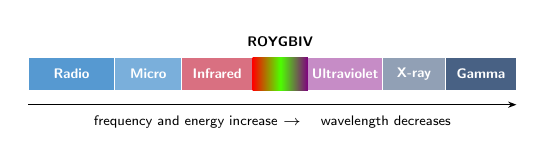
\begin{tikzpicture}[x=1cm, y=1cm, font=\tiny\sffamily]
  \foreach \x/\w/\l/\c in {0/1.1/Radio/dblue!70, 1.1/0.85/Micro-/dblue!55, 1.95/0.9/Infrared/rosered!70, 2.85/0.7/Visible/white, 3.55/0.95/Ultraviolet/violet!45, 4.5/0.8/X-ray/dnavy!45, 5.3/0.9/Gamma/dnavy!75}{
    \fill[\c] (\x,0) rectangle ++(\w,0.42);
    \draw[white] (\x,0) rectangle ++(\w,0.42);}
  \shade[left color=red, right color=violet, middle color=green!70!yellow] (2.85,0) rectangle (3.55,0.42);
  \foreach \x/\w/\l in {0/1.1/Radio, 1.1/0.85/Micro, 1.95/0.9/Infrared, 3.55/0.95/Ultraviolet, 4.5/0.8/X-ray, 5.3/0.9/Gamma}
    \node[white, font=\tiny\sffamily\bfseries] at (\x+\w/2,0.21) {\l};
  \node[font=\tiny\sffamily\bfseries] at (3.2,0.62) {ROYGBIV};
  \draw[-{Stealth[length=3pt]}] (0,-0.18) -- (6.2,-0.18);
  \node[anchor=north] at (3.1,-0.2) {frequency and energy increase $\rightarrow$ \quad wavelength decreases};
\end{tikzpicture}
\figcap{The electromagnetic spectrum. All EM waves travel at $c=3\times10^8$ m/s in vacuum.}
\end{center}
\begin{itemize}
\item Uses: radio (broadcasting), microwaves (cooking, phones, radar), infrared (remote controls, thermal cameras), visible, UV (sterilizing, vitamin D, sunburn), X-rays (bones), gamma (cancer therapy, sterilizing tools). Red has the longest visible wavelength, violet the shortest.
\item \term{Reflection}: angle of incidence $=$ angle of reflection, both measured from the \textbf{normal}. Plane mirror image: virtual, upright, same size, as far behind as the object is in front, left--right reversed. Two mirrors at angle $\theta$ make $\frac{360}{\theta}-1$ images. Two mirrors at 90$^\circ$ send a ray back parallel to where it came from.
\item \term{Concave mirror} (converging): object beyond $C$ $\to$ real, inverted, smaller; \textbf{at $C=2f$ $\to$ real, inverted, same size}; between $F$ and the mirror $\to$ virtual, upright, magnified (makeup mirror). \term{Convex mirror}: always virtual, upright, smaller (side mirrors, store mirrors).
\item \term{Refraction}: light bends \textbf{toward} the normal entering a denser medium (higher $n$) and away from it leaving. $n=\frac cv$; Snell: $n_1\sin\theta_1=n_2\sin\theta_2$. Water 1.33, glass $\approx$ 1.5, diamond 2.42.
\item \term{Total internal reflection}: going from dense to less dense beyond the critical angle, $\sin\theta_c=\frac{n_2}{n_1}$ (optical fibers, diamond sparkle, mirages). A prism disperses white light; violet bends most.
\item \term{Convex (converging) lens}: object inside $F$ $\to$ virtual, upright, enlarged (magnifying glass); farther out $\to$ real, inverted (camera, eye). Corrects farsightedness. \term{Concave lens}: always virtual, upright, smaller; corrects nearsightedness.
\item Mirror and lens equation $\frac1f=\frac1{d_o}+\frac1{d_i}$; magnification $m=-\frac{d_i}{d_o}$. Real images have $d_i>0$.
\item Primary colors of light: red, green, blue (R $+$ G $=$ yellow; all three $=$ white). The sky is blue because short wavelengths scatter more; sunsets are red.
\end{itemize}

\sub{H. Electricity}
\begin{formbox}
$I=\dfrac Qt$ \textbullet\ Ohm's law $V=IR$ \textbullet\ $P=VI=I^2R=\dfrac{V^2}R$ \textbullet\ energy $=Pt$ (kWh)\\
Series $R=R_1+R_2+\cdots$ \textbullet\ Parallel $\dfrac1R=\dfrac1{R_1}+\dfrac1{R_2}+\cdots$ ($n$ equal resistors: $\frac Rn$) \textbullet\ wire $R=\rho\dfrac LA$
\end{formbox}
\begin{itemize}
\item Series: same current, voltages add, one break stops everything. Parallel: same voltage, currents add, the total resistance is smaller than the smallest branch; one bulb out leaves the rest on (holiday lights that stay lit when one bulb is removed are in parallel).
\item Longer or thinner wire $\Rightarrow$ more resistance; hotter metal $\Rightarrow$ more resistance. Ammeters go in series, voltmeters in parallel.
\item A 1{,}000-W appliance used 3 h uses 3 kWh. Philippine outlets: 220 V AC, 60 Hz. Fuses and breakers protect against overloads.
\item Like charges repel. Charging by friction, conduction, or induction. Coulomb: $F=\frac{kq_1q_2}{r^2}$.
\end{itemize}

\sub{I. Magnetism and electromagnetism}
Field lines run from N to S outside a magnet. A current makes a magnetic field (Oersted). \term{Electromagnet}: more turns, more current, iron core $\Rightarrow$ stronger (attracts more nails). \term{Motor}: electrical $\to$ mechanical. \term{Generator}: mechanical $\to$ electrical, by \emph{electromagnetic induction} (Faraday: a changing magnetic field induces a voltage). \term{Transformer}: $\frac{V_s}{V_p}=\frac{N_s}{N_p}$, AC only.

% ============================================================ SPACE SCIENCE
\sect{9}{Space Science}

\sub{A. The universe and stars}
\begin{itemize}
\item \term{Big Bang}: about 13.8 billion years ago. Evidence: galaxies are moving away (redshift; Hubble), the cosmic microwave background, the abundance of hydrogen and helium.
\item Galaxies: spiral (the \textbf{Milky Way}, a barred spiral; Andromeda), elliptical, irregular. The Sun is one of hundreds of billions of stars in the Milky Way.
\item Stars form in \textbf{nebulae}, shine by \textbf{fusing hydrogen into helium}. A Sun-like star: main sequence $\to$ red giant $\to$ planetary nebula $\to$ \textbf{white dwarf}. A massive star: red supergiant $\to$ \textbf{supernova} $\to$ neutron star or black hole.
\item Color shows surface temperature: \textbf{blue} (hottest) $\to$ white $\to$ yellow (the Sun, about 5{,}500$^\circ$C) $\to$ orange $\to$ \textbf{red} (coolest). Spectral classes O B A F G K M. The H--R diagram plots brightness against temperature.
\item Nearest star: the Sun; next, Proxima Centauri (about 4.2 light-years). Polaris (North Star) marks north; the Southern Cross is seen from the Philippines in the south.
\end{itemize}
\begin{keybox}[Units]
A \textbf{light-year} is a \emph{distance} (how far light travels in a year, $\approx9.46\times10^{12}$ km), not a time. 1 AU $\approx$ 150 million km (Earth--Sun distance). Sunlight takes about 8 minutes to reach us.
\end{keybox}

\sub{B. The Sun}
Core (fusion, about 15 million $^\circ$C) $\to$ radiative zone $\to$ convective zone $\to$ \textbf{photosphere} (visible surface; \textbf{sunspots} are cooler, darker areas on an 11-year cycle) $\to$ chromosphere $\to$ \textbf{corona} (outer atmosphere, seen in a total solar eclipse). Solar flares and coronal mass ejections cause auroras and can disrupt satellites and power grids.

\sub{C. The solar system}
{\footnotesize\renewcommand{\arraystretch}{1.04}
\begin{tabularx}{\linewidth}{@{}>{\leavevmode\bfseries\color{dnavy}}p{0.55in}L@{}}
\toprule
Mercury & smallest planet, closest to the Sun, shortest year (88 days), almost no atmosphere\\
Venus & \textbf{hottest} planet (thick CO$_2$ greenhouse), spins backward, brightest planet in our sky\\
Earth & liquid water, life; densest planet\\
Mars & red (iron oxide); Olympus Mons, the largest volcano; moons Phobos and Deimos\\
Jupiter & \textbf{largest} and most massive; Great Red Spot; moon Ganymede is the largest moon\\
Saturn & brightest rings; least dense (would float on water); moon Titan has a thick atmosphere\\
Uranus & tilted on its side ($\approx98^\circ$); blue-green from methane\\
Neptune & farthest; strongest winds\\\bottomrule
\end{tabularx}}
\begin{itemize}
\item Order: \textbf{M}y \textbf{V}ery \textbf{E}ducated \textbf{M}other \textbf{J}ust \textbf{S}erved \textbf{U}s \textbf{N}achos. Inner (terrestrial) planets are small and rocky; outer (Jovian) planets are gas and ice giants with rings and many moons.
\item Pluto was reclassified as a \textbf{dwarf planet} in 2006 because it has not cleared its orbital neighborhood. Other dwarf planets: Ceres (asteroid belt), Eris, Haumea, Makemake.
\item Asteroid belt: between Mars and Jupiter. Kuiper belt: beyond Neptune. Comets are icy; their tails point \emph{away from the Sun} (Halley's comet returns about every 76 years). Meteoroid (in space) $\to$ meteor (streak of light) $\to$ meteorite (lands on Earth).
\end{itemize}
\begin{formbox}[Kepler's laws]
(1) Orbits are ellipses with the Sun at one focus. (2) A planet sweeps equal areas in equal times, so it moves \textbf{fastest when closest} (perihelion). (3) $T^2\propto a^3$: farther planets have longer years.
\end{formbox}

\sub{D. Earth, Moon, and Sun}
\begin{itemize}
\item \term{Rotation} (24 h): day and night; the Sun appears to rise in the east because Earth spins west to east. \term{Revolution} (365\textonequarter\ days): hence leap years.
\item \term{Seasons} come from the \textbf{23.5$^\circ$ tilt} of Earth's axis, not from distance (Earth is closest to the Sun in early January). June solstice: longest day in the Northern Hemisphere; December solstice: shortest; March and September equinoxes: equal day and night. The Philippines, in the tropics, has wet and dry seasons instead.
\item Moon phases (29.5 days): new $\to$ waxing crescent $\to$ first quarter $\to$ waxing gibbous $\to$ full $\to$ waning gibbous $\to$ third quarter $\to$ waning crescent. The Moon shines by reflected sunlight and keeps the same face toward Earth.
\item \term{Solar eclipse}: Moon between Sun and Earth, only at \textbf{new moon}. \term{Lunar eclipse}: Earth between Sun and Moon, only at \textbf{full moon} (the Moon may look red). Not monthly, because the Moon's orbit is tilted about 5$^\circ$.
\item \term{Tides} come mainly from the Moon's pull. Spring tides (largest range) at new and full moon, when Sun, Earth, and Moon line up; neap tides (smallest) at the quarter moons.
\end{itemize}

\sub{E. Exploring space}
Sputnik 1 (1957, first satellite) \textbullet\ Yuri Gagarin (1961, first human in space) \textbullet\ Apollo 11 (1969, Neil Armstrong, first on the Moon) \textbullet\ Hubble Space Telescope (1990) \textbullet\ International Space Station \textbullet\ James Webb Space Telescope (infrared, launched 2021) \textbullet\ Voyager 1 (in interstellar space). The Philippines: \textbf{Diwata-1} (2016), the first Philippine microsatellite, built by Filipino engineers under a DOST program; \textbf{Maya-1} (2018), the first Philippine cubesat; the \textbf{Philippine Space Agency} (PhilSA) was created in 2019. Telescopes: refracting (lenses) vs.\ reflecting (mirrors). Astronauts in orbit feel weightless because they are in continuous free fall.

% ============================================================ MATHEMATICS
\sect{10}{Mathematics}

Algebra, Geometry, Trigonometry, Statistics, and Calculus (70 minutes, the longest part). Assume \textbf{no calculator}: factor before you multiply, and look for the trick that keeps numbers small.

\sub{A. Number sense}
\begin{itemize}
\item Divisibility: 3 and 9 (digit sum), 4 (last two digits), 8 (last three), 11 (alternating sum). Primes below 50: 2 3 5 7 11 13 17 19 23 29 31 37 41 43 47.
\item $\text{GCF}\times\text{LCM}=$ product of the two numbers. If $N=p^aq^br^c$, it has $(a+1)(b+1)(c+1)$ positive divisors.
\item Percent: ``25\% of $s$ is 20'' $\Rightarrow s=80$. $x\%$ of $y$ $=$ $y\%$ of $x$. If 70\% of a fee is subsidized and you pay PhP\,500 per unit, the 500 is \emph{your} 30\%: for 3 units, $1500=0.30T\Rightarrow T=5000$, so the government pays PhP\,3{,}500. Always ask what each number is a percent \emph{of}.
\item Ratio and proportion: map scale $\frac14$ in : 20 ft $\Rightarrow$ 50 ft is $\frac{50}{20}\times\frac14=\frac58$ in.
\end{itemize}

\sub{B. Algebra essentials}
\begin{formbox}[Exponents, radicals, factoring]
$a^ma^n=a^{m+n}$ \textbullet\ $(a^m)^n=a^{mn}$ \textbullet\ $a^{-n}=\frac1{a^n}$ \textbullet\ $a^{m/n}=\sqrt[n]{a^m}$ \textbullet\ $a^0=1$\\
$(a\pm b)^2=a^2\pm2ab+b^2$ \textbullet\ $a^2-b^2=(a+b)(a-b)$ \textbullet\ $a^3\pm b^3=(a\pm b)(a^2\mp ab+b^2)$\\
Rationalize: $\dfrac{1}{\sqrt a-\sqrt b}=\dfrac{\sqrt a+\sqrt b}{a-b}$
\end{formbox}
\begin{itemize}
\item \term{Inequalities}: flip the sign when multiplying or dividing by a negative. $|x-a|<b\iff a-b<x<a+b$; $|x-a|>b\iff x<a-b$ or $x>a+b$.
\item \term{Systems}: substitution or elimination. Parallel lines (same slope, different intercept) have no solution.
\item \term{Variation}: direct $y=kx$; inverse $y=\frac kx$; joint $y=kxz$.
\item \term{Remainder theorem}: $P(x)\div(x-a)$ leaves remainder $P(a)$; if $P(a)=0$, $(x-a)$ is a factor.
\item Complex numbers: $i^2=-1$; powers of $i$ repeat every 4 ($i,-1,-i,1$).
\end{itemize}

\sub{C. Quadratics and functions}
\begin{formbox}[Quadratics]
$x=\dfrac{-b\pm\sqrt{b^2-4ac}}{2a}$ \textbullet\ discriminant $b^2-4ac$: $>0$ two real, $=0$ one (double), $<0$ none real\\
Sum of roots $=-\frac ba$ \textbullet\ product $=\frac ca$ \textbullet\ vertex at $x=-\frac b{2a}$
\end{formbox}
\begin{itemize}
\item \term{Domain}: no zero denominators, no negative under an even root, log arguments $>0$.
\item \term{Composition} $(f\circ g)(x)=f(g(x))$: work from the inside out. \term{Inverse}: swap $x$ and $y$, solve for $y$; $f^{-1}(b)=a$ means $f(a)=b$.
\item \term{Transformations}: $f(x-h)+k$ moves the graph right $h$, up $k$; $-f(x)$ reflects across the $x$-axis; $f(-x)$ across the $y$-axis.
\item \term{Writing a rule from a table}: check differences. Math 100, 90, 50\ldots\ vs.\ History 90, 80, 40\ldots: every History score is 10 less, so $Y=X-10$ (Primer).
\end{itemize}

\sub{D. Exponentials and logarithms}
\begin{formbox}[Logs]
$\log_bx=y\iff b^y=x$ \textbullet\ $\log_b(xy)=\log_bx+\log_by$ \textbullet\ $\log_b\frac xy=\log_bx-\log_by$ \textbullet\ $\log_bx^n=n\log_bx$\\
$\log_bb=1$, $\log_b1=0$ \textbullet\ change of base $\log_bx=\dfrac{\log x}{\log b}$ \textbullet\ growth/decay $A=A_0\,b^{t/T}$
\end{formbox}
Write both sides with the same base: $8^{x-1}=4^{x+1}\Rightarrow2^{3x-3}=2^{2x+2}\Rightarrow x=5$. Always check log solutions: arguments must stay positive. Bacteria $b=b_0(3^{-2t})$ with $b_0=2700$, $t=1$: $2700\cdot\frac19=300$.

\sub{E. Sequences and series}
\begin{formbox}[Progressions]
Arithmetic: $a_n=a_1+(n-1)d$; $S_n=\frac n2(a_1+a_n)$\\
Geometric: $a_n=a_1r^{n-1}$; $S_n=\dfrac{a_1(r^n-1)}{r-1}$; infinite sum $\dfrac{a_1}{1-r}$ for $|r|<1$
\end{formbox}
A ball dropped from 16 ft that rises to 2 ft after the third bounce: $16r^3=2\Rightarrow r=\frac12$.

\sub{F. Analytic geometry and conics}
\begin{itemize}
\item Slope $m=\frac{y_2-y_1}{x_2-x_1}$; $y=mx+b$; $y-y_1=m(x-x_1)$. Parallel: equal slopes. Perpendicular: $m_1m_2=-1$. Distance $\sqrt{(\Delta x)^2+(\Delta y)^2}$; midpoint $\left(\frac{x_1+x_2}2,\frac{y_1+y_2}2\right)$; point to line $\dfrac{|Ax_0+By_0+C|}{\sqrt{A^2+B^2}}$.
\item \term{Circle} $(x-h)^2+(y-k)^2=r^2$. From the general form, complete the square: $x^2+y^2-6x+4y-12=0\Rightarrow(x-3)^2+(y+2)^2=25$.
\item \term{Parabola} $(x-h)^2=4p(y-k)$: focus $p$ units from the vertex. \term{Ellipse} $\frac{x^2}{a^2}+\frac{y^2}{b^2}=1$, $c^2=a^2-b^2$. \term{Hyperbola} $\frac{x^2}{a^2}-\frac{y^2}{b^2}=1$, $c^2=a^2+b^2$, asymptotes $y=\pm\frac bax$.
\item Identify $Ax^2+Cy^2+Dx+Ey+F=0$: $A=C$ circle; $A,C$ same sign ellipse; opposite signs hyperbola; one of them 0 parabola.
\end{itemize}
\begin{dost}[Primer Math item 1]
$2(x+1)^2+(y-2)^2=25$ and $4(x+1)^2-3(y-2)^2=15$. Let $u=(x+1)^2$, $v=(y-2)^2$: $2u+v=25$, $4u-3v=15\Rightarrow u=9$, $v=7$. Then $x+1=\pm3$ and $y-2=\pm\sqrt7$: \textbf{4} intersection points (an ellipse meets a hyperbola).
\end{dost}

\sub{G. Geometry}
\begin{itemize}
\item Angles: complementary 90$^\circ$, supplementary 180$^\circ$, vertical angles equal. Parallel lines and a transversal: corresponding and alternate interior angles are equal; same-side interior angles are supplementary.
\item Triangles: angles sum to 180$^\circ$; an exterior angle equals the two remote interior angles; any side is less than the sum of the other two. 30-60-90 sides $1:\sqrt3:2$; 45-45-90 sides $1:1:\sqrt2$. Triples: 3-4-5, 5-12-13, 8-15-17, 7-24-25.
\item \term{Similar figures}: if sides are in ratio $k$, areas are in $k^2$ and volumes in $k^3$.
\item Polygons: interior angle sum $(n-2)180^\circ$; exterior sum 360$^\circ$; each exterior angle of a regular $n$-gon $=\frac{360^\circ}n$; diagonals $\frac{n(n-3)}2$.
\item Areas: triangle $\frac12bh=\frac12ab\sin C$; Heron's formula $\sqrt{s(s-a)(s-b)(s-c)}$ with $s=\frac{a+b+c}2$; equilateral $\frac{\sqrt3}4s^2$; parallelogram $bh$; trapezoid $\frac12(b_1+b_2)h$; rhombus $\frac12d_1d_2$; circle $\pi r^2$; sector $\frac\theta{360}\pi r^2$; arc $\frac\theta{360}2\pi r$.
\item \term{Pick's theorem} (dot grids): area $=I+\frac B2-1$ ($I$ interior dots, $B$ boundary dots). Or split the shape into rectangles and triangles.
\item Volumes: prism/cylinder $Bh$, $\pi r^2h$; pyramid/cone $\frac13Bh$, $\frac13\pi r^2h$; sphere $\frac43\pi r^3$, surface $4\pi r^2$. A cone holds $\frac13$ of the cylinder with the same base and height.
\end{itemize}
\begin{formbox}[Circle angle and segment rules]
Central angle $=$ its arc \textbullet\ inscribed angle $=\frac12$ arc (in a semicircle: 90$^\circ$)\\
Two chords meeting \emph{inside}: angle $=\frac12$(sum of the two intercepted arcs)\\
Secants/tangents meeting \emph{outside}: angle $=\frac12$(difference of the arcs)\\
Chords: $(AE)(EB)=(CE)(ED)$ \textbullet\ tangent $\perp$ radius \textbullet\ two tangents from one point are equal\\
Opposite angles of a cyclic quadrilateral are supplementary
\end{formbox}
\begin{dost}[Primer Math item 3]
Arc $CD=(x-3)^\circ$, arc $AB=(3x+11)^\circ$. $\angle CMD=\frac12[(x-3)+(3x+11)]=\frac12(4x+8)=\mathbf{2x+4}$.
\end{dost}

\sub{H. Trigonometry}
SOH--CAH--TOA; $\csc=\frac1{\sin}$, $\sec=\frac1{\cos}$, $\cot=\frac1{\tan}$; $\pi$ rad $=180^\circ$; arc length $s=r\theta$ ($\theta$ in radians).\par
{\footnotesize\renewcommand{\arraystretch}{1.25}\centering
\begin{tabular}{@{}c|ccccc@{}}
 & $0^\circ$ & $30^\circ$ & $45^\circ$ & $60^\circ$ & $90^\circ$\\\hline
$\sin$ & 0 & $\frac12$ & $\frac{\sqrt2}2$ & $\frac{\sqrt3}2$ & 1\\
$\cos$ & 1 & $\frac{\sqrt3}2$ & $\frac{\sqrt2}2$ & $\frac12$ & 0\\
$\tan$ & 0 & $\frac{\sqrt3}3$ & 1 & $\sqrt3$ & undef.\\
\end{tabular}\par}
\begin{formbox}[Identities and triangle laws]
$\sin^2\theta+\cos^2\theta=1$ \textbullet\ $1+\tan^2\theta=\sec^2\theta$ \textbullet\ $1+\cot^2\theta=\csc^2\theta$\\
$\sin(A\pm B)=\sin A\cos B\pm\cos A\sin B$ \textbullet\ $\cos(A\pm B)=\cos A\cos B\mp\sin A\sin B$\\
$\sin2A=2\sin A\cos A$ \textbullet\ $\cos2A=\cos^2A-\sin^2A=1-2\sin^2A$\\
Law of sines $\dfrac a{\sin A}=\dfrac b{\sin B}$ \textbullet\ law of cosines $c^2=a^2+b^2-2ab\cos C$
\end{formbox}
\begin{itemize}
\item Signs by quadrant (``All Students Take Calculus''): QI all positive, QII sin, QIII tan, QIV cos.
\item $y=A\sin(Bx+C)+D$: amplitude $|A|$, period $\frac{2\pi}{|B|}$.
\item Angle of elevation (looking up) $=$ angle of depression (looking down) between the same two points.
\end{itemize}

\sub{I. Statistics}
\begin{itemize}
\item Mean $\bar x=\frac{\sum x}n$; missing value $=$ (new $n$)(new mean) $-$ (old sum). Median: middle of the sorted data. Mode: most frequent.
\item Range, variance $s^2=\frac{\sum(x-\bar x)^2}{n-1}$, standard deviation $s$. Small SD $=$ data bunched near the mean.
\item Adding $c$ to every value shifts the mean, median, and mode by $c$ but leaves the range and SD \textbf{unchanged}. Multiplying by $k$ multiplies the mean and SD by $k$.
\item $z=\dfrac{x-\mu}{\sigma}$ compares scores from different tests. Normal curve: 68\% within 1 SD, 95\% within 2, 99.7\% within 3.
\item Correlation $r$ from $-1$ to $1$: near $\pm1$ strong, near 0 weak; correlation is not causation.
\end{itemize}
\begin{center}
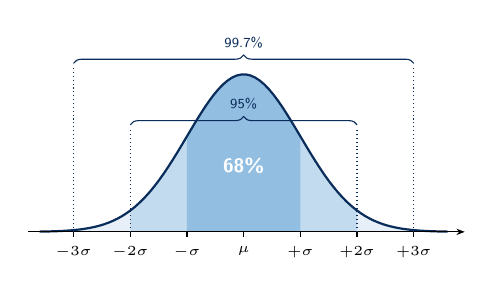
\begin{tikzpicture}[x=0.72cm, y=2.0cm, font=\tiny\sffamily]
  \fill[dblue!10] plot[domain=-3:3, samples=60] (\x,{exp(-0.5*(\x)*(\x))}) -- (3,0) -- (-3,0) -- cycle;
  \fill[dblue!25] plot[domain=-2:2, samples=50] (\x,{exp(-0.5*(\x)*(\x))}) -- (2,0) -- (-2,0) -- cycle;
  \fill[dblue!45] plot[domain=-1:1, samples=40] (\x,{exp(-0.5*(\x)*(\x))}) -- (1,0) -- (-1,0) -- cycle;
  \draw[dnavy, thick] plot[domain=-3.6:3.6, samples=90] (\x,{exp(-0.5*(\x)*(\x))});
  \draw[-{Stealth[length=3pt]}] (-3.8,0) -- (3.9,0);
  \foreach \k/\l in {-3/{$-3\sigma$}, -2/{$-2\sigma$}, -1/{$-\sigma$}, 0/{$\mu$}, 1/{$+\sigma$}, 2/{$+2\sigma$}, 3/{$+3\sigma$}}
    {\draw (\k,0) -- (\k,-0.03) node[below] {\l};}
  \node[white, font=\scriptsize\sffamily\bfseries] at (0,0.42) {68\%};
  \draw[dnavy, decorate, decoration={brace, amplitude=3pt}] (-2,0.68) -- (2,0.68) node[midway, above=2pt] {95\%};
  \draw[dnavy, decorate, decoration={brace, amplitude=3pt}] (-3,1.07) -- (3,1.07) node[midway, above=2pt] {99.7\%};
  \draw[dnavy, densely dotted] (-2,0) -- (-2,0.66) (2,0) -- (2,0.66) (-3,0) -- (-3,1.05) (3,0) -- (3,1.05);
\end{tikzpicture}
\figcap{The empirical rule for a normal distribution.}
\end{center}

\sub{J. Counting and probability}
\begin{formbox}[Counting]
Multiply choices at each stage \textbullet\ permutations (order matters) $_nP_r=\dfrac{n!}{(n-r)!}$ \textbullet\ combinations (order doesn't) $_nC_r=\dfrac{n!}{r!(n-r)!}$\\
Circular arrangements $(n-1)!$ \textbullet\ letters with repeats $\dfrac{n!}{a!\,b!\cdots}$
\end{formbox}
\begin{itemize}
\item $P(E)=\frac{\text{favorable}}{\text{total}}$; $P(\text{not }E)=1-P(E)$; $P(A\cup B)=P(A)+P(B)-P(A\cap B)$; independent: $P(A\cap B)=P(A)P(B)$; conditional: $P(A|B)=\frac{P(A\cap B)}{P(B)}$.
\item Two dice: 36 outcomes; ways to get sums 2--12: 1, 2, 3, 4, 5, \textbf{6}, 5, 4, 3, 2, 1. Cards: 52, four suits of 13, 12 face cards.
\item ``At least one'' $=1-P(\text{none})$. Coins: $n$ coins give $2^n$ outcomes.
\end{itemize}
\begin{dost}[Primer Math item 2]
Chips 1--10, draw two: $\binom{10}2=45$ pairs; one even and one odd: $5\times5=25$. $P=\frac{25}{45}=\mathbf{\frac59}$.
\end{dost}

\sub{K. Calculus}
\begin{itemize}
\item \term{Limits}: substitute first; if you get $\frac00$, factor and cancel: $\lim_{x\to2}\frac{x^2-4}{x-2}=\lim_{x\to2}(x+2)=4$. $\lim_{x\to0}\frac{\sin x}x=1$. At infinity, compare the highest powers (equal degrees: ratio of leading coefficients). L'H\^opital: for $\frac00$ or $\frac\infty\infty$, differentiate top and bottom.
\item The derivative $f'(x)$ is the slope of the tangent line, the instantaneous rate of change. Motion: $v=s'$, $a=v'=s''$.
\end{itemize}
\begin{formbox}[Derivatives]
$(x^n)'=nx^{n-1}$ \textbullet\ $(c)'=0$ \textbullet\ $(uv)'=u'v+uv'$ \textbullet\ $\left(\frac uv\right)'=\dfrac{u'v-uv'}{v^2}$ \textbullet\ chain: $[f(g(x))]'=f'(g(x))\,g'(x)$\\
$(\sin x)'=\cos x$ \textbullet\ $(\cos x)'=-\sin x$ \textbullet\ $(\tan x)'=\sec^2x$ \textbullet\ $(e^x)'=e^x$ \textbullet\ $(\ln x)'=\frac1x$
\end{formbox}
\begin{itemize}
\item \term{Critical points}: $f'(x)=0$. Second-derivative test: $f''<0$ local max, $f''>0$ local min. $f''$ changes sign at an inflection point.
\item \term{Optimization}: write the quantity in one variable, set the derivative to 0. With a fixed perimeter, the rectangle of greatest area is a square.
\item Tangent line at $x=a$: $y-f(a)=f'(a)(x-a)$.
\end{itemize}
\begin{formbox}[Integrals]
$\int x^ndx=\dfrac{x^{n+1}}{n+1}+C$ ($n\neq-1$) \textbullet\ $\int\frac1xdx=\ln|x|+C$ \textbullet\ $\int e^xdx=e^x+C$\\
$\int\sin x\,dx=-\cos x+C$ \textbullet\ $\int\cos x\,dx=\sin x+C$ \textbullet\ $\int_a^bf(x)dx=F(b)-F(a)$ $=$ net area under the curve
\end{formbox}

% ============================================================ PRIMER DECODED
\sect{11}{The Primer's sample items, explained}

The official 2026 Primer gives answers without explanations. Here is the reasoning for each one, with page numbers from the Primer (figures are in the Primer itself).

\sub{Mechanical Reasoning (p.~6)}
\ans{1}{C}{The bus accelerates left, so the soda ``lags'' and piles up at the back (right). The surface tilts up toward the right: the choice whose line rises to the right.}
\ans{2}{B}{Kite II, the simple diamond, has the most sail area for its weight and the least drag, so it climbs highest fastest. The boxy kite I and the bulkier kite III carry more weight and drag for their size.}
\ans{3}{\textit{see note}}{W and X are in parallel, and that pair is in series with the pair Y and Z. If Y burns out, the circuit's resistance rises from $R$ to $\frac32R$, so the battery current falls to $\frac23$ of its old value. W and X each carry $\frac13I_0$ instead of $\frac12I_0$ (dimmer); Z carries $\frac23I_0$ instead of $\frac12I_0$ (brighter). That is \textbf{II and III} (choice \textbf{C}). The Primer's key says B (I and IV), which would mean Z dims while W and X brighten; that does not follow from the circuit as drawn. If this item appears on your exam, reason it out the way shown here.}

\sub{Spatial Reasoning (pp.~7--8)}
\ans{1}{C}{3, 4, ?, 6, 7 sides: the missing shape has 5 sides, the pentagon.}
\ans{2}{B}{Folding along both dashed lines stacks the four quarters on the top-left one. The top-left hole stays at the top left. The bottom-right quarter is flipped twice (a 180$^\circ$ turn), so its hole, near that quarter's top-left corner, lands at the \emph{bottom right}. Two holes, diagonal: B.}
\ans{3}{B}{Count the regions in each choice (there must be exactly five) and match each region to a piece by its angles and relative size, starting with the two triangles. The choice where every piece fits with no gaps is B.}
\ans{4}{C}{Pick one distinctive feature, the sloping back, and note what it touches (which end, which side the legs are on). A true rotation keeps those neighbors in the same arrangement; choices that swap sides are mirror images. That leaves C.}

\sub{Verbal Reasoning (p.~9)}
\ans{1}{D}{A lifebelt is a safety device for the sea; a \emph{parachute} is one for the air. (The pair's order is reversed in the stem: read it as SEA : LIFEBELT :: AIR : PARACHUTE.)}
\ans{2}{B}{Anterior and posterior are opposites: front and \emph{hind} (back).}
\ans{3}{C}{The root \emph{geo} means earth; \emph{ferro} means \emph{iron} (ferrous, ferromagnetic).}
\ans{4}{D}{Newton developed calculus; Copernicus contributed to \emph{astronomy} (the heliocentric model). Astrology is not a science.}
\ans{5}{B}{A hammer is the carpenter's main tool; a brush is the painter's. A blueprint is the architect's product, not a tool.}
\ans{6}{C}{Infatuation is an excessive, foolish form of affection; cowardice is an excessive form of timidity (both nouns).}

\sub{Language and Literature (pp.~10--11)}
\ans{1}{C}{Faulty parallelism: ``picked up\ldots, \emph{straightened} her hat grimly, and took\ldots'' The \emph{-ing} form breaks the series of past-tense verbs.}
\ans{2}{A}{\emph{Shy} and \emph{effusive} (gushing, very expressive) are opposites; the other pairs are synonyms.}
\ans{3}{C}{\emph{Sometime} $=$ at an unspecified point in time (``sometime next month''). \emph{Some time} is a span of time.}
\ans{4}{A}{``Do you mind\ldots?'' asks whether it bothers you; ``Not at all'' means ``no, I'll gladly do it.''}
\ans{5}{B}{The passage calls the koala a marsupial ``associated to wombats.''}
\ans{6}{C}{``Rest during the day and become active only at night'' defines \emph{nocturnal}.}
\ans{7}{B}{``Their fur keeps them warm during the cold season.''}
\ans{8}{C}{``Having a keen sense of smell, they are able to differentiate\ldots''}

\sub{Science (pp.~12--13)}
\ans{1}{D}{Legume bacteria add nitrogen to the soil. Plan D grows mongo in 4 of 6 years (A and C have 3, B only 1), so it adds the most nitrogen.}
\ans{2}{B}{Combined gas law in kelvins: $T_2=308\times1.6=492.8$ K $\approx$ 220$^\circ$C (worked in Section 6H).}
\ans{3}{C}{Without air resistance, the motion is symmetric: same height, same speed. At Z the velocity is horizontal, not zero, and the acceleration is still $g$. Y and W have equal speeds but different directions.}
\ans{4}{D}{Geothermal energy is heat from magma beneath the surface.}
\ans{5}{C}{I (angle of incidence) and II (atmospheric absorption over different path lengths) explain the latitude difference; III is about time, not latitude.}
\ans{6}{B}{Jupiter.}

\sub{Mathematics (pp.~13--14)}
\ans{1}{D}{4 points (Section 10F).}
\ans{2}{C}{$\frac{25}{45}=\frac59$ (Section 10J).}
\ans{3}{B}{$2x+4$ (Section 10G).}
\ans{4}{B}{Each History score is the Math score minus 10: $Y=X-10$.}

\begin{caution}[If you also use SYENSIYA-bilidad (2013)]
A few answers in that book's key don't match their own solutions. \textbf{I.B-10}: after the power stroke comes the \emph{exhaust} stroke (B), not intake. \textbf{II.A-18}: the independent variable is the \emph{type of medium} (B), as its own explanation says. \textbf{II.B-13}: its solution computes the 79$^\circ$ launch (choice C), not 83$^\circ$. \textbf{II.B-20}: $1.8\to0.028$ g/m$^2$ is about 6 half-lives $=6\times1000\approx6.01\times10^3$ days (C). The rest of the book is still great practice for figure memory, robot paths, and organ pathways.
\end{caution}

\end{multicols}

% =====================================================================
%                              MOCK EXAM
% =====================================================================
\newpage
\begin{tcolorbox}[enhanced, colback=dnavy, colframe=dnavy, boxrule=0pt, arc=4pt,
  left=12pt, right=12pt, top=6pt, bottom=6pt, before skip=0pt, after skip=4pt]
{\sffamily\bfseries\footnotesize\color{dgold}PRACTICE TEST \textbullet\ 100 ITEMS \textbullet\ 3 PARTS \textbullet\ 130 MINUTES}\par\vspace{1pt}
{\sffamily\bfseries\LARGE\color{white}Mock DOST-SEI Scholarship Exam}\hfill{\sffamily\bfseries\color{dgold}\atom[dgold]\ Iskolar ng Agham!}\par\vspace{1pt}
{\sffamily\color{white}\footnotesize Modeled on the domains and item styles of the 2026 Primer. All passages and questions are original.}
\end{tcolorbox}

\begin{tcolorbox}[enhanced, colback=dmist, colframe=dblue!55, boxrule=0.5pt, arc=2pt,
  left=6pt, right=6pt, top=3pt, bottom=3pt, before skip=0pt, after skip=4pt, fontupper=\footnotesize]
\textbf{\sffamily\color{dblue}Directions.} Each item has four choices. Choose the \textbf{best} answer and shade its letter on the answer sheet (page after the test). No calculator, phone, or notes; scratch paper is fine. Time each part separately and do not go back to a finished part, just like the real exam: \textbf{Part I} (items 1--35) 35 minutes, \textbf{Part II} (items 36--70) 45 minutes, \textbf{Part III} (items 71--100) 50 minutes. Use $g=9.8$ m/s$^2$ unless an item says otherwise. In error-identification items, choose the underlined part that contains the error. For syllogisms, use only the given statements.
\end{tcolorbox}

\begin{multicols}{2}

% ------------------------------------------------------------ PART I
\parthead{PART I}{Reasoning, Language \& Literature}{1--35 \textbullet\ 35 min}

\subhead{Mechanical Reasoning}
\begin{enumerate}[series=exam, label=\textbf{\arabic*.}, leftmargin=1.95em, itemsep=4pt]

\item A glass of water sits in a cup holder of a car moving \emph{east}. The driver brakes hard. While the car is slowing down, the water surface
\optgrid{stays level.}{rises on the east side.}{rises on the west side.}{bulges up in the middle.}

\item A 600-N rock rests on a crowbar 0.5 m from the fulcrum. What effort, applied 1.5 m from the fulcrum on the other side, will just balance it?
\optrow{200 N}{300 N}{900 N}{1800 N}

\item Five gears are meshed in a straight line, numbered 1 to 5. Gear 1 has 40 teeth and turns clockwise at 30 rpm. Gear 5 has 20 teeth. How does gear 5 turn?
\optgrid{clockwise, 15 rpm}{counterclockwise, 60 rpm}{clockwise, 60 rpm}{counterclockwise, 15 rpm}

\item In a block and tackle, four rope segments support the movable pulley. Ignoring friction, what effort lifts an 800-N load, and how much rope must be pulled to raise the load 1 m?
\optgrid{200 N; 1 m of rope}{200 N; 4 m of rope}{800 N; 4 m of rope}{400 N; 2 m of rope}

\item Identical bulbs P and Q are connected in parallel, and this pair is connected in series with an identical bulb R across a battery. If bulb Q burns out, what happens to P and R?
\optlist{P gets dimmer and R gets brighter.}{Both P and R get brighter.}{Both P and R go out.}{P gets brighter and R gets dimmer.}

\item Three small holes are punched, one above another, on the side of a tall plastic bottle full of water. From which hole does water spurt out fastest?
\optgrid{the top hole}{the middle hole}{the bottom hole}{all three equally}

\item During a typhoon, strong wind sometimes lifts the roof off a house even though the wind blows sideways. The best explanation is that
\optlist{fast-moving air above the roof has lower pressure than the still air inside the house.}{the wind pushes down on the roof harder than on the walls.}{the heated roof expands and pops off its nails.}{the air inside the house cools and pulls the roof upward.}

\item Four identical bottles each hold the same amount of sand. Which is LEAST likely to tip over when bumped?
\optlist{standing upright, with the sand settled at the bottom}{standing upside down on its cap, with the sand settled in the neck}{standing upright, with the sand stuck to the inside near the top}{standing upside down on its cap, with the sand stuck near the (now upturned) bottom}

% ------------------------------------------------------------ spatial
\end{enumerate}
\subhead{Spatial Reasoning}
\begin{enumerate}[resume*=exam]

\item Which figure comes next in the series?\par
\begin{center}
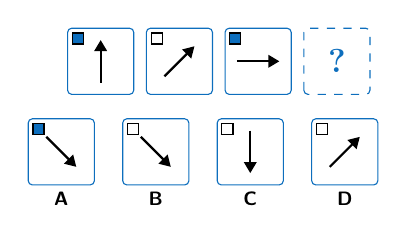
\begin{tikzpicture}[font=\scriptsize\sffamily]
  \newcommand{\arframe}[3]{%
    \begin{scope}[shift={(#1,0)}]
      \draw[dblue, rounded corners=1.5pt] (-0.42,-0.42) rectangle (0.42,0.42);
      \draw[thick, -{Triangle[length=4pt, width=4.5pt]}] ($(0,0)+(#2+180:0.27)$) -- ($(0,0)+(#2:0.27)$);
      \draw[black, fill=#3] (-0.36,0.22) rectangle (-0.22,0.36);
    \end{scope}}
  \arframe{0}{90}{dblue}
  \arframe{1}{45}{white}
  \arframe{2}{0}{dblue}
  \draw[dblue, rounded corners=1.5pt, dashed] (2.58,-0.42) rectangle (3.42,0.42);
  \node[font=\large\bfseries, dblue] at (3,0) {?};
  \begin{scope}[yshift=-1.15cm, xshift=-0.5cm]
    \arframe{0}{-45}{dblue}
    \arframe{1.2}{-45}{white}
    \arframe{2.4}{-90}{white}
    \arframe{3.6}{45}{white}
    \foreach \x/\l in {0/A, 1.2/B, 2.4/C, 3.6/D} \node[font=\scriptsize\sffamily\bfseries] at (\x,-0.6) {\l};
  \end{scope}
\end{tikzpicture}
\end{center}

\item A square sheet of paper is folded in half along its vertical center line, left half onto right half. A hole is then punched through both layers near the folded sheet's upper-right corner. When the sheet is unfolded, where are the holes?
\optlist{near the upper-left and upper-right corners}{near the upper-right and lower-right corners}{one hole, near the upper-right corner only}{side by side, near the middle of the top edge}

\item The net below is folded into a cube. Which face is opposite face 1?\par
\begin{center}
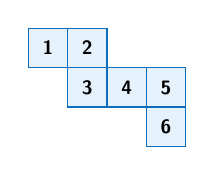
\begin{tikzpicture}[x=0.5cm, y=0.5cm, font=\scriptsize\sffamily\bfseries]
  \foreach \x/\y/\l in {0/1/1, 1/1/2, 1/0/3, 2/0/4, 3/0/5, 3/-1/6}{
    \draw[dblue, fill=dice] (\x,\y) rectangle ++(1,1);
    \node at (\x+0.5,\y+0.5) {\l};}
\end{tikzpicture}
\end{center}
\optrow{2}{3}{6}{4}

\item On a standard die, which two numbers can NEVER be seen at the same time?
\optrow{1 and 2}{2 and 6}{4 and 5}{3 and 4}

\item A card printed with the word {\sffamily\bfseries GRAVITY} stands upright facing a plane mirror. Which shows its image in the mirror?\par
\vspace{2pt}{\sffamily\bfseries\renewcommand{\arraystretch}{1.3}\setlength{\tabcolsep}{0pt}%
\begin{tabular}{@{}p{0.5\linewidth}p{0.5\linewidth}@{}}
\textmd{A.}~\reflectbox{GRAVITY} & \textmd{B.}~\rotatebox[origin=c]{180}{GRAVITY}\\
\textmd{C.}~\rotatebox[origin=c]{180}{\reflectbox{GRAVITY}} & \textmd{D.}~YTIVARG
\end{tabular}}

\item Which is a ROTATION (not a mirror image) of the letter-shape {\sffamily\bfseries\large F}?\par
\vspace{2pt}{\sffamily\bfseries\Large\setlength{\tabcolsep}{0pt}%
\begin{tabular}{@{}*{4}{p{0.25\linewidth}}@{}}
{\normalsize\textmd{A.}}~\reflectbox{F} & {\normalsize\textmd{B.}}~\rotatebox[origin=c]{180}{F} & {\normalsize\textmd{C.}}~\rotatebox[origin=c]{180}{\reflectbox{F}} & {\normalsize\textmd{D.}}~\rotatebox[origin=c]{90}{\reflectbox{F}}
\end{tabular}}

\item A $4\times4\times4$ cube is painted on all its faces, then cut into 64 unit cubes. How many unit cubes have paint on exactly two faces?
\optrow{8}{16}{24}{36}

% ------------------------------------------------------------ verbal
\end{enumerate}
\subhead{Verbal Reasoning}
\begin{enumerate}[resume*=exam]

\item HYDRO : WATER :: PYRO : \underline{\hspace{1.2cm}}
\optrow{air}{stone}{light}{fire}

\item LAVOISIER : CONSERVATION OF MASS :: MENDEL : \underline{\hspace{1.2cm}}
\optgrid{evolution by natural selection}{the periodic table}{laws of inheritance}{the cell theory}

\item THERMOMETER : TEMPERATURE ::\\ ANEMOMETER :~\underline{\hspace{1.2cm}}
\optgrid{air pressure}{humidity}{wind direction}{wind speed}

\item WARM : HOT ::
\optgrid{cold : ice}{drizzle : downpour}{rain : cloud}{fast : slow}

\item All metals conduct electricity. Some solids are metals. Which statement must be true?
\optlist{All solids conduct electricity.}{No solid conducts electricity.}{All conductors are metals.}{Some solids conduct electricity.}

\item Ana is taller than Ben. Carlo is shorter than Ben. Dina is taller than Ana. Who is the second tallest?
\optrow{Ana}{Ben}{Carlo}{Dina}

\item What comes next? \quad B, \ E, \ I, \ N, \ \underline{\hspace{0.6cm}}
\optrow{S}{R}{T}{U}

% ------------------------------------------------------------ language
\end{enumerate}
\subhead{Language and Literature}
\begin{enumerate}[resume*=exam]

\item Which underlined part shows an ERROR?\\
Each of the students \err{who joined}{A} the science fair \err{have submitted}{B} \err{a research paper}{C} \err{to the panel}{D} before the deadline.
\optrow{A}{B}{C}{D}

\item Which underlined part shows an ERROR?\\
\err{Between you and I}{A}, the results of the experiment \err{were}{B} \err{more surprising}{C} than \err{we expected}{D}.
\optrow{A}{B}{C}{D}

\item Which underlined part shows an ERROR?\\
The volunteers \err{sorted the donations}{A}, \err{packed them}{B}, \err{and were delivering them}{C} \err{to the evacuees}{D}.
\optrow{A}{B}{C}{D}

\item Her research findings will greatly \underline{\hspace{1.2cm}} the way farmers manage their crops.
\optrow{effect}{effects}{affects}{affect}

\item The laboratory has \underline{\hspace{1.2cm}} microscopes than the school needs.
\optrow{fewer}{less}{lesser}{least}

\item Which is the most appropriate response that \emph{grants} the request?\\
\emph{``Would you mind if I borrowed your calculator?''}
\optgrid{``Yes, I would. Here it is.''}{``Not at all. Go ahead.''}{``Yes, please.''}{``No, you can't mind.''}

\item Which pair of words are ANTONYMS?
\optgrid{candid -- frank}{frugal -- thrifty}{verbose -- terse}{amiable -- friendly}

\item ``After weeks of review, the final exam was a \emph{piece of cake} for Lia.'' The idiom means the exam was
\optgrid{very easy.}{a reward.}{a celebration.}{very difficult.}

\item ``The wind whispered secrets through the bamboo grove.'' This line uses
\optgrid{simile.}{personification.}{hyperbole.}{onomatopoeia.}

\item Which work by Jos\'e Rizal is the sequel to \emph{Noli Me T\'angere}?
\optgrid{\emph{Florante at Laura}}{\emph{El Filibusterismo}}{``Mi \'Ultimo Adi\'os''}{\emph{Dekada '70}}
\end{enumerate}

\begin{passage}{Passage \textbullet\ for items 33--35}
In the 1880s, the German psychologist Hermann Ebbinghaus ran an unusual experiment on the only subject he could fully control: himself. He memorized long lists of nonsense syllables such as DAX, BUP, and ZOL, chosen precisely because they meant nothing, so that nothing he already knew could help him. Then he tested how much he still remembered after minutes, hours, and days.

The results traced what is now called the \emph{forgetting curve}. Memory dropped steeply at first, with much of a list gone within a day, and then declined more slowly. Ebbinghaus also noticed something more hopeful: each time he relearned a list, he needed less effort, and the list faded more slowly afterward.

Today this finding underlies \emph{spaced repetition}, the practice of reviewing material at gradually lengthening intervals. A student who reviews a lesson the next day, again after three days, and again after a week will usually remember far more than one who rereads it five times the night before an exam. Cramming can feel productive, but much of what is crammed quickly evaporates.
\end{passage}

\begin{enumerate}[resume*=exam]
\item Which best states the main idea of the passage?
\optlist{Ebbinghaus preferred nonsense syllables to real words.}{Memory declines at a constant rate over time.}{Students should never study the night before an exam.}{Research on forgetting shows that spaced review helps memory more than cramming.}

\item As used in the last sentence, \emph{evaporates} most nearly means
\optgrid{turns into vapor.}{becomes clearer.}{is quickly forgotten.}{spreads to others.}

\item Why did Ebbinghaus use nonsense syllables?
\optlist{to make the experiment entertaining}{because they were shorter than real words}{to keep what he already knew from helping him remember}{to test other people's memories}
\end{enumerate}

% ------------------------------------------------------------ PART II
\parthead{PART II}{Science}{36--70 \textbullet\ 45 min}

\subhead{Biology}
\begin{enumerate}[resume*=exam]
\item Red blood cells are placed in distilled water. What happens to them?
\optgrid{They shrivel (crenate).}{They stay the same.}{They swell and may burst.}{They lose their nuclei.}

\item In pea plants, tall (T) is dominant over short (t). Two heterozygous tall plants are crossed. What fraction of the offspring is expected to be short?
\optrow{0}{$\frac14$}{$\frac12$}{$\frac34$}

\item Red--green color blindness is X-linked recessive. A color-blind man marries a woman who is homozygous for normal vision. What is expected of their children?
\optlist{All of the sons will be color-blind.}{Half of the daughters will be color-blind.}{All of the children will be color-blind.}{All daughters will be carriers with normal vision; all sons will have normal vision.}

\item A DNA template strand reads 3$'$--TACGGATTC--5$'$. Which mRNA (written 5$'$ to 3$'$) is transcribed from it?
\optgrid{AUGCCUAAG}{ATGCCTAAG}{UACGGAUUC}{AUGGCUAAG}

\item A human cell with 46 chromosomes undergoes meiosis. The result is
\optlist{four cells, each with 23 chromosomes.}{two cells, each with 46 chromosomes.}{four cells, each with 46 chromosomes.}{two cells, each with 23 chromosomes.}

\item In the food chain grass $\to$ grasshopper $\to$ frog $\to$ snake, the grass stores 10{,}000 kJ of energy. Using the 10\% rule, about how much reaches the snake?
\optrow{1{,}000 kJ}{100 kJ}{10 kJ}{1 kJ}

\item \emph{Rhizobium} bacteria live in the root nodules of legumes. They fix nitrogen for the plant and receive sugars in return. This relationship is
\optgrid{parasitism.}{commensalism.}{mutualism.}{predation.}

\item A bat's wing, a whale's flipper, and a human arm have the same arrangement of bones but different functions. They are examples of
\optgrid{analogous structures.}{homologous structures.}{vestigial structures.}{mutations.}
\end{enumerate}

\subhead{Chemistry}
\begin{enumerate}[resume*=exam]
\item How many neutrons are in an atom of $^{56}_{26}$Fe?
\optrow{26}{30}{56}{82}

\item Which element has the highest electronegativity?
\optrow{Na}{Cl}{F}{I}

\item What is the molecular shape of ammonia, NH$_3$?
\optgrid{trigonal planar}{tetrahedral}{bent}{trigonal pyramidal}

\item Aluminum ions (Al$^{3+}$) combine with sulfate ions (SO$_4^{2-}$). The formula of the compound is
\optrow{AlSO$_4$}{Al$_2$(SO$_4$)$_3$}{Al$_3$(SO$_4$)$_2$}{Al(SO$_4$)$_3$}

\item What is the mass of 0.50 mol of CO$_2$? (C $=12$, O $=16$)
\optrow{22 g}{11 g}{44 g}{88 g}

\item A balloon holds 2.0 L of gas at 27$^\circ$C. At constant pressure, what is its volume at 127$^\circ$C?
\optrow{2.7 L}{9.4 L}{1.5 L}{2.0 L}

\item Solution X has pH 3 and solution Y has pH 5. Which statement is true?
\optlist{Y is more acidic than X.}{X has twice the hydrogen-ion concentration of Y.}{X has 100 times the hydrogen-ion concentration of Y.}{Both solutions are basic.}

\item Using the activity series K $>$ Na $>$ Mg $>$ Zn $>$ Fe $>$ (H) $>$ Cu $>$ Ag, which reaction will NOT occur?
\optlist{Zn $+$ CuSO$_4$ $\to$ ZnSO$_4$ $+$ Cu}{Mg $+$ 2HCl $\to$ MgCl$_2$ $+$ H$_2$}{Fe $+$ 2AgNO$_3$ $\to$ Fe(NO$_3$)$_2$ $+$ 2Ag}{Cu $+$ ZnSO$_4$ $\to$ CuSO$_4$ $+$ Zn}
\end{enumerate}

\subhead{Earth Science}
\begin{enumerate}[resume*=exam]
\item S waves are not detected on the side of Earth opposite an earthquake. This ``shadow zone'' shows that
\optlist{the inner core is liquid.}{the outer core is liquid.}{the crust is thickest under the oceans.}{the mantle is made mostly of iron.}

\item The Philippine Trench, east of Mindanao and the Visayas, formed where
\optlist{two continental plates collide.}{two plates pull apart.}{two plates slide past each other horizontally.}{an oceanic plate sinks beneath another plate.}

\item Which statement about earthquakes is correct?
\optlist{Magnitude measures the energy released; intensity describes the effects at a particular place.}{Intensity is the same everywhere the earthquake is felt.}{Magnitude is reported using the PHIVOLCS Earthquake Intensity Scale.}{The epicenter is the point deep underground where the rupture begins.}

\item Marble forms when limestone is changed by heat and pressure. Marble is therefore
\optgrid{an igneous rock.}{a sedimentary rock.}{a metamorphic rock.}{a mineral, not a rock.}

\item In which layer of the atmosphere does almost all weather occur?
\optgrid{troposphere}{stratosphere}{mesosphere}{thermosphere}

\item On a sunny afternoon at the beach, the wind usually blows
\optlist{from land to sea, because the sea is warmer.}{parallel to the shore.}{from sea to land, because the land heats up faster and the air above it rises.}{from land to sea, because land is denser than water.}

\item In the Philippines, \emph{Habagat} refers to
\optlist{the northeast monsoon, which brings cool, dry air.}{El Ni\~no.}{a tropical cyclone with winds above 185 km/h.}{the southwest monsoon, which brings heavy rains.}
\end{enumerate}

\subhead{Physics}
\begin{enumerate}[resume*=exam]
\item A ball is thrown at an angle above level ground. Ignoring air resistance, at the highest point of its path
\optlist{its velocity and acceleration are both zero.}{its velocity is zero, but its acceleration is 9.8 m/s$^2$ downward.}{its velocity is horizontal, and its acceleration is 9.8 m/s$^2$ downward.}{its velocity is horizontal, and its acceleration is zero.}

\item A 5.0-kg cart is pulled with a 30-N force while 10 N of friction acts on it. What is its acceleration?
\optrow{2 m/s$^2$}{4 m/s$^2$}{6 m/s$^2$}{8 m/s$^2$}

\item A stone is dropped from rest from a bridge and hits the water 3.0 s later. About how high is the bridge?
\optrow{14.7 m}{29.4 m}{88.2 m}{44.1 m}

\item A 2-kg ball is dropped from a height of 5 m. Using $g=10$ m/s$^2$, what is its speed just before it hits the ground?
\optrow{10 m/s}{5 m/s}{50 m/s}{100 m/s}

\item Three 6-$\Omega$ resistors are connected in parallel across a 12-V battery. What is the total current from the battery?
\optrow{0.67 A}{2 A}{18 A}{6 A}

\item An object stands 30 cm in front of a concave mirror whose focal length is 10 cm. Where is the image, and what kind is it?
\optlist{15 cm from the mirror; real and inverted}{15 cm behind the mirror; virtual and upright}{7.5 cm from the mirror; real and inverted}{20 cm behind the mirror; virtual and upright}

\item A student shouts toward a cliff and hears the echo 2.0 s later. If sound travels at 340 m/s, how far away is the cliff?
\optrow{170 m}{340 m}{680 m}{1{,}360 m}
\end{enumerate}

\subhead{Space Science}
\begin{enumerate}[resume*=exam]
\item Which planet is the hottest, even though it is not the closest to the Sun?
\optrow{Mercury}{Venus}{Mars}{Jupiter}

\item A solar eclipse can happen only during which phase of the Moon?
\optgrid{full moon}{first quarter}{new moon}{third quarter}

\item A light-year is a unit of
\optrow{distance.}{time.}{brightness.}{speed.}

\item Earth has seasons mainly because
\optlist{Earth's distance from the Sun changes greatly during the year.}{Earth's axis is tilted about 23.5$^\circ$.}{the Sun's energy output changes with the seasons.}{the Moon blocks part of the sunlight.}

\item Which star has the hottest surface?
\optrow{a red star}{an orange star}{a yellow star}{a blue-white star}
\end{enumerate}

% ------------------------------------------------------------ PART III
\parthead{PART III}{Mathematics}{71--100 \textbullet\ 50 min}

\begin{enumerate}[resume*=exam]
\item Simplify $(2x^3y^{-2})^2\cdot3xy^5$.
\optrow{$12x^7y$}{$6x^7y$}{$12x^6y^3$}{$12x^7y^9$}

\item For what values of $k$ does $x^2+kx+9=0$ have exactly one real root?
\optrow{$\pm3$}{$\pm6$}{$\pm9$}{$\pm18$}

\item The sum of two numbers is 30 and their difference is 8. What is their product?
\optrow{209}{221}{189}{240}

\item If $f(x)=2x-3$ and $g(x)=x^2$, find $f(g(3))-g(f(3))$.
\optrow{0}{6}{9}{15}

\item If $f(x)=\dfrac{3x+1}{2}$, what is $f^{-1}(5)$?
\optrow{8}{2}{$\frac73$}{3}

\item Solve $\log_2(x+3)+\log_2(x-3)=4$.
\optgrid{$x=-5$ and $x=5$}{$x=5$ only}{$x=8$}{$x=-5$ only}

\item The first term of a geometric sequence is 3 and the fourth term is 81. What is the sum of the first five terms?
\optrow{243}{363}{364}{729}

\item What is the sum of all positive multiples of 7 that are less than 100?
\optrow{700}{742}{805}{735}

\item What are the center and radius of $x^2+y^2-6x+4y-12=0$?
\optgrid{$(3,-2)$; 5}{$(-3,2)$; 5}{$(3,-2)$; 25}{$(-3,2)$; $\sqrt{12}$}

\item The graph of $4x^2-9y^2-16x+18y-29=0$ is
\optgrid{a circle.}{a parabola.}{an ellipse.}{a hyperbola.}

\item Each interior angle of a regular polygon measures 144$^\circ$. How many sides does it have?
\optrow{8}{9}{10}{12}

\item Chords $AB$ and $CD$ of a circle intersect at $E$. If $AE=4$, $EB=6$, and $CE=3$, find $ED$.
\optrow{4.5}{6}{8}{12}

\item An inscribed angle intercepts an arc of 110$^\circ$. What is the measure of the angle?
\optrow{55$^\circ$}{110$^\circ$}{220$^\circ$}{70$^\circ$}

\item Two similar triangles have corresponding sides in the ratio $2:3$. The smaller triangle's area is 24 cm$^2$. What is the larger triangle's area?
\optrow{36 cm$^2$}{48 cm$^2$}{54 cm$^2$}{72 cm$^2$}

\item A cone and a cylinder have the same radius and the same height. The cylinder's volume is $81\pi$ cm$^3$. What is the cone's volume?
\optrow{$9\pi$}{$27\pi$}{$40.5\pi$}{$243\pi$}

\item Which line passes through $(1,2)$ and is perpendicular to $y=2x+5$?
\optgrid{$x+2y=5$}{$2x-y=0$}{$x-2y=-3$}{$2x+y=4$}

\item If $\sin\theta=\frac35$ and $\theta$ is in Quadrant II, find $\cos\theta+\tan\theta$.
\optrow{$-\frac{31}{20}$}{$\frac{31}{20}$}{$-\frac1{20}$}{$\frac1{20}$}

\item Simplify $(1+\tan^2\theta)\cos^2\theta$.
\optrow{$\sin^2\theta$}{$1$}{$\tan^2\theta$}{$\sec^2\theta$}

\item Two sides of a triangle are 5 and 8, and the angle between them is 60$^\circ$. How long is the third side?
\optrow{6}{$\sqrt{89}$}{9}{7}

\item From a point 30 m from the base of a tree on level ground, the angle of elevation of the treetop is 60$^\circ$. How tall is the tree?
\optrow{$10\sqrt3$ m}{15 m}{$30\sqrt3$ m}{60 m}

\item The mean of five numbers is 18. When a sixth number is added, the mean becomes 20. What is the sixth number?
\optrow{20}{22}{30}{38}

\item Every score in a data set is increased by 5 points. Which statement is true?
\optlist{The mean and the standard deviation both increase by 5.}{The mean increases by 5; the standard deviation is unchanged.}{The mean is unchanged; the standard deviation increases by 5.}{Both the mean and the standard deviation are unchanged.}

\item Ana scored 85 on a test with mean 75 and standard deviation 5. Ben scored 80 on a test with mean 70 and standard deviation 10. Who did better relative to the class?
\optlist{Ana, because her $z$-score is 2}{Ben, because his $z$-score is 1}{They did equally well, since both scored 10 above the mean.}{It cannot be determined.}

\item Two fair dice are rolled. What is the probability that the sum is 9?
\optrow{$\frac1{12}$}{$\frac19$}{$\frac16$}{$\frac5{36}$}

\item In how many ways can a president, a vice president, and a secretary be chosen from 7 students?
\optrow{35}{21}{343}{210}

\item Evaluate $\displaystyle\lim_{x\to2}\frac{x^2-4}{x-2}$.
\optrow{0}{2}{4}{does not exist}

\item If $f(x)=3x^4-2x^2+7$, find $f'(1)$.
\optrow{8}{12}{16}{6}

\item At what value of $x$ does $f(x)=x^3-3x$ have a local maximum?
\optrow{1}{0}{$-1$}{$\sqrt3$}

\item A farmer has 100 m of fencing to enclose a rectangular garden. What is the largest area he can enclose?
\optrow{400 m$^2$}{500 m$^2$}{2{,}500 m$^2$}{625 m$^2$}

\item Evaluate $\displaystyle\int_0^2(3x^2+2x)\,dx$.
\optrow{8}{10}{16}{12}
\end{enumerate}

\vfill
\begin{center}
{\sffamily\bfseries\color{dblue}--- END OF MOCK EXAM ---}\\[1pt]
{\footnotesize\sffamily Stop the timer. Finish shading the answer sheet before you look at the key.}
\end{center}

\end{multicols}

% =====================================================================
%                              ANSWER SHEET
% =====================================================================
\newpage
\begin{tcolorbox}[enhanced, colback=dnavy, colframe=dnavy, boxrule=0pt, arc=4pt,
  left=12pt, right=12pt, top=5pt, bottom=5pt, before skip=0pt, after skip=6pt]
{\sffamily\bfseries\Large\color{white}Mock Exam Answer Sheet}\hfill{\sffamily\bfseries\color{dgold}\atom[dgold]\ Shade one circle per item}
\end{tcolorbox}

{\sffamily\small Name \rule{2.6in}{0.4pt}\hfill Date \rule{1.1in}{0.4pt}\hfill Start \rule{0.7in}{0.4pt}\hfill End \rule{0.7in}{0.4pt}}
\vspace{8pt}

\begin{center}
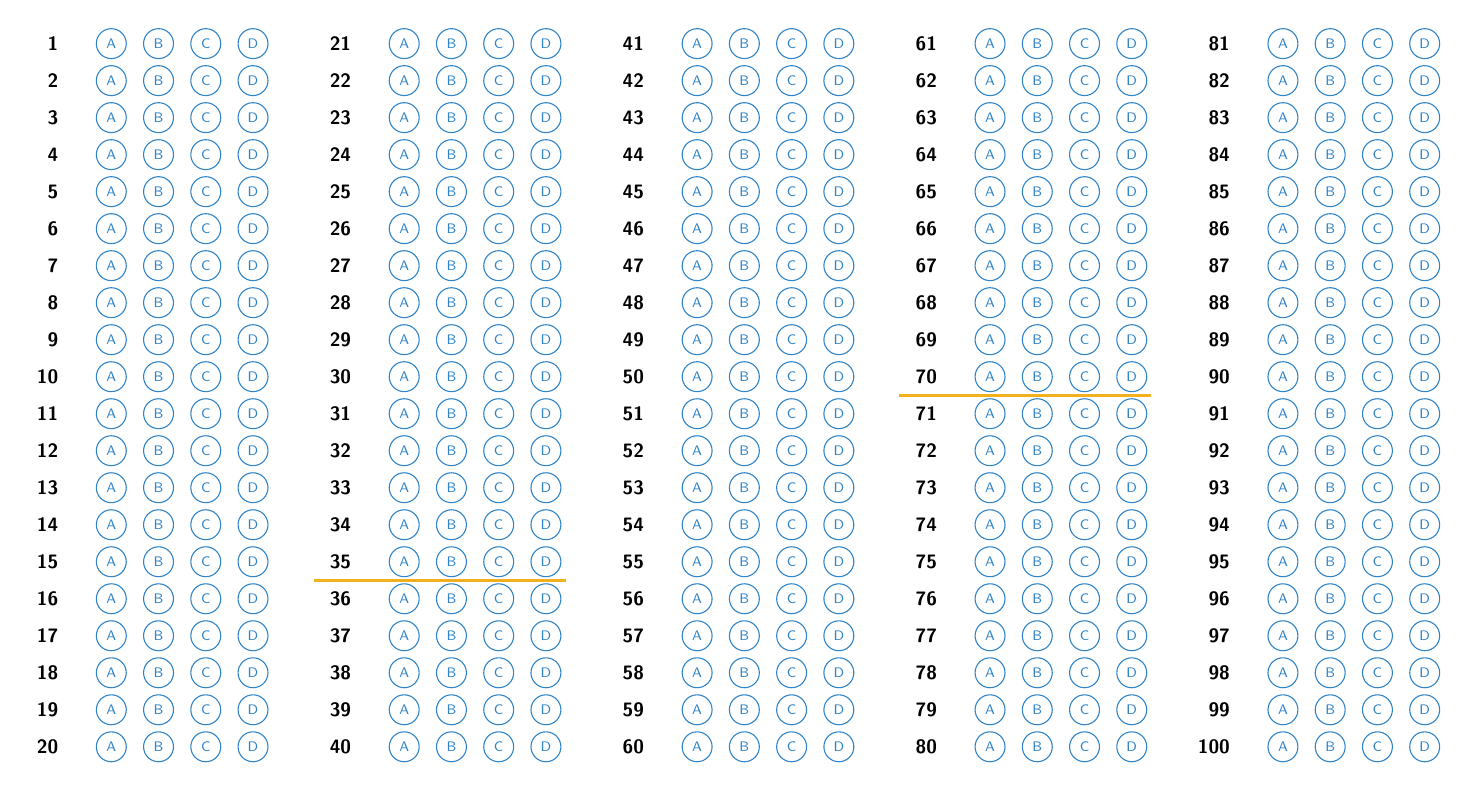
\begin{tikzpicture}[x=1cm, y=1cm]
  \foreach \c in {0,...,4}{
    \foreach \r in {1,...,20}{
      \pgfmathtruncatemacro{\n}{\c*20+\r}
      \node[anchor=east, font=\scriptsize\sffamily\bfseries] at (\c*3.72+0.25, -\r*0.47) {\n};
      \foreach \L [count=\i] in {A,B,C,D}{
        \draw[dblue!85] (\c*3.72+0.2+\i*0.6, -\r*0.47) circle (0.19);
        \node[dblue!85, font=\fontsize{5.5}{6}\selectfont\sffamily] at (\c*3.72+0.2+\i*0.6, -\r*0.47) {\L};
      }
    }
  }
  % part boundaries: after items 35 and 70
  \foreach \c/\r in {1/15, 3/10}
    \draw[dgold, very thick] (\c*3.72-0.35, -\r*0.47-0.235) -- (\c*3.72+2.85, -\r*0.47-0.235);
\end{tikzpicture}
\end{center}
{\centering\scriptsize\sffamily\color{dgold!55!black}Gold lines mark the end of each part: I (1--35) \textbullet\ II (36--70) \textbullet\ III (71--100)\par}
\vspace{8pt}

\begin{center}
\begin{tcolorbox}[enhanced, width=6.4in, colback=dmist, colframe=dblue!55, boxrule=0.5pt, arc=2pt,
  left=6pt, right=6pt, top=3pt, bottom=3pt, before skip=0pt, after skip=0pt]
{\sffamily\bfseries\color{dblue}Score yourself}\par\vspace{2pt}
{\footnotesize\renewcommand{\arraystretch}{1.2}\centering
\newcommand{\blank}{\rule{0.45in}{0.4pt}}
\begin{tabular}{@{}l l c c | l l c c@{}}
\toprule
Domain & Items & Total & Correct & Domain & Items & Total & Correct\\\midrule
Mechanical Reasoning & 1--8 & 8 & \blank & Biology & 36--43 & 8 & \blank\\
Spatial Reasoning & 9--15 & 7 & \blank & Chemistry & 44--51 & 8 & \blank\\
Verbal Reasoning & 16--22 & 7 & \blank & Earth Science & 52--58 & 7 & \blank\\
Language \& Literature & 23--35 & 13 & \blank & Physics & 59--65 & 7 & \blank\\
\textbf{Part I total} & & \textbf{35} & \blank & Space Science & 66--70 & 5 & \blank\\
Algebra & 71--80 & 10 & \blank & \textbf{Part II total} & & \textbf{35} & \blank\\
Geometry & 81--86 & 6 & \blank & & & & \\
Trigonometry & 87--90 & 4 & \blank & & & & \\
Statistics \& Probability & 91--95 & 5 & \blank & & & & \\
Calculus & 96--100 & 5 & \blank & & & & \\
\textbf{Part III total} & & \textbf{30} & \blank & \textbf{GRAND TOTAL} & & \textbf{100} & \blank\\\bottomrule
\end{tabular}\par}
\vspace{3pt}
{\footnotesize\textbf{85--100} Scholar-ready: keep this pace on exam day. \textbullet\ \textbf{70--84} Solid: reread the sections for any domain below 70\%. \textbullet\ \textbf{50--69} Getting there: redo the boxes in your two weakest domains, then retake those items. \textbullet\ \textbf{Below 50}: go for the fastest points first: the formula boxes in Sections 6--8 and 10, and the analogy and functional-English rules in Sections 3--4. \emph{This is a practice score, not a DOST-SEI score; the real exam's difficulty and cut-off are not published.}\par}
\end{tcolorbox}
\end{center}

% =====================================================================
%                              ANSWER KEY
% =====================================================================
\newpage
\begin{tcolorbox}[enhanced, colback=dnavy, colframe=dnavy, boxrule=0pt, arc=4pt,
  left=12pt, right=12pt, top=5pt, bottom=5pt, before skip=0pt, after skip=5pt]
{\sffamily\bfseries\Large\color{white}Answer Key \& Solutions}\hfill{\sffamily\bfseries\color{dgold}\atom[dgold]\ Check, then reread what you missed}
\end{tcolorbox}

\newcommand{\kk}[2]{\textbf{#1}\,\textcolor{dblue}{\textbf{#2}}}
{\small\centering\renewcommand{\arraystretch}{1.2}\setlength{\tabcolsep}{5.6pt}
\begin{tabular}{@{}*{10}{l}@{}}
\rowcolor{dice}\kk{1}{B}&\kk{2}{A}&\kk{3}{C}&\kk{4}{B}&\kk{5}{D}&\kk{6}{C}&\kk{7}{A}&\kk{8}{A}&\kk{9}{B}&\kk{10}{A}\\
\kk{11}{D}&\kk{12}{D}&\kk{13}{A}&\kk{14}{B}&\kk{15}{C}&\kk{16}{D}&\kk{17}{C}&\kk{18}{D}&\kk{19}{B}&\kk{20}{D}\\
\rowcolor{dice}\kk{21}{A}&\kk{22}{C}&\kk{23}{B}&\kk{24}{A}&\kk{25}{C}&\kk{26}{D}&\kk{27}{A}&\kk{28}{B}&\kk{29}{C}&\kk{30}{A}\\
\kk{31}{B}&\kk{32}{B}&\kk{33}{D}&\kk{34}{C}&\kk{35}{C}&\kk{36}{C}&\kk{37}{B}&\kk{38}{D}&\kk{39}{A}&\kk{40}{A}\\
\rowcolor{dice}\kk{41}{C}&\kk{42}{C}&\kk{43}{B}&\kk{44}{B}&\kk{45}{C}&\kk{46}{D}&\kk{47}{B}&\kk{48}{A}&\kk{49}{A}&\kk{50}{C}\\
\kk{51}{D}&\kk{52}{B}&\kk{53}{D}&\kk{54}{A}&\kk{55}{C}&\kk{56}{A}&\kk{57}{C}&\kk{58}{D}&\kk{59}{C}&\kk{60}{B}\\
\rowcolor{dice}\kk{61}{D}&\kk{62}{A}&\kk{63}{D}&\kk{64}{A}&\kk{65}{B}&\kk{66}{B}&\kk{67}{C}&\kk{68}{A}&\kk{69}{B}&\kk{70}{D}\\
\kk{71}{A}&\kk{72}{B}&\kk{73}{A}&\kk{74}{B}&\kk{75}{D}&\kk{76}{B}&\kk{77}{B}&\kk{78}{D}&\kk{79}{A}&\kk{80}{D}\\
\rowcolor{dice}\kk{81}{C}&\kk{82}{C}&\kk{83}{A}&\kk{84}{C}&\kk{85}{B}&\kk{86}{A}&\kk{87}{A}&\kk{88}{B}&\kk{89}{D}&\kk{90}{C}\\
\kk{91}{C}&\kk{92}{B}&\kk{93}{A}&\kk{94}{B}&\kk{95}{D}&\kk{96}{C}&\kk{97}{A}&\kk{98}{C}&\kk{99}{D}&\kk{100}{D}\\
\end{tabular}\par}
\vspace{5pt}

\begin{multicols}{2}
\footnotesize
\setlength{\parskip}{1.6pt}

{\sffamily\bfseries\color{dblue}Part I \textbullet\ Mechanical Reasoning}
\ans{1}{B}{Braking means the acceleration points west, so the water keeps moving east and piles up at the front: the east side.}
\ans{2}{A}{$600(0.5)=F(1.5)\Rightarrow F=200$ N.}
\ans{3}{C}{Odd-numbered gears turn like gear 1 (clockwise). Middle gears don't change the ratio: $40\times30=20\times\text{rpm}\Rightarrow60$ rpm.}
\ans{4}{B}{MA $=4$: effort $=\frac{800}4=200$ N; work in $=$ work out, so $200\times d=800\times1\Rightarrow d=4$ m.}
\ans{5}{D}{Before: $R_\text{total}=\frac R2+R=1.5R$. After Q opens: P and R are simply in series, $2R$. Current drops from $\frac V{1.5R}$ to $\frac V{2R}$, so R (which carries all of it) dims. P's current rises from half of $\frac V{1.5R}=\frac V{3R}$ to $\frac V{2R}$: brighter.}
\ans{6}{C}{Pressure $\rho gh$ is greatest at the greatest depth.}
\ans{7}{A}{Bernoulli: fast air above the roof means lower pressure; the higher pressure inside pushes the roof up.}
\ans{8}{A}{Lowest center of gravity on the widest base. B, C, D put the base on the narrow cap or the sand up high.}

{\sffamily\bfseries\color{dblue}Part I \textbullet\ Spatial Reasoning}
\ans{9}{B}{The arrow turns 45$^\circ$ clockwise each step (up, up-right, right, \emph{down-right}); the small square alternates filled, empty, filled, \emph{empty}.}
\ans{10}{A}{The folded sheet is the right half, so its upper-right corner is the sheet's upper-right corner. Unfolding mirrors the hole across the center line to the upper left.}
\ans{11}{D}{Fold with 3 as the base: 2 becomes the back, 1 (attached to 2) the left side, 4 the right side, 5 the top, and 6 the front. Left (1) is opposite right (4). Also 3--5 and 2--6.}
\ans{12}{D}{Opposite faces of a die add to 7, and you can never see two opposite faces at once: 3 and 4.}
\ans{13}{A}{A vertical mirror reverses left and right: the whole word is flipped horizontally (letters and order). C is a water (top--bottom) image; B is a 180$^\circ$ turn.}
\ans{14}{B}{A 180$^\circ$ turn keeps the shape's handedness. A and C are reflections; D is a reflection followed by a rotation, which is still a mirror image.}
\ans{15}{C}{Two painted faces sit along the 12 edges, minus the corners: $12(4-2)=24$.}

{\sffamily\bfseries\color{dblue}Part I \textbullet\ Verbal Reasoning}
\ans{16}{D}{Hydro means water; pyro means fire (pyrotechnics).}
\ans{17}{C}{Lavoisier is known for the law of conservation of mass; Mendel for the laws of inheritance.}
\ans{18}{D}{A thermometer measures temperature; an anemometer measures wind \emph{speed}. A wind vane gives direction.}
\ans{19}{B}{Hot is a stronger degree of warm; a downpour is a stronger degree of drizzle.}
\ans{20}{D}{The solids that are metals must conduct, so at least some solids conduct. The other choices go beyond the statements.}
\ans{21}{A}{Dina $>$ Ana $>$ Ben $>$ Carlo.}
\ans{22}{C}{B2, E5, I9, N14: $+3,+4,+5$, so next is $14+6=20$, T.}

{\sffamily\bfseries\color{dblue}Part I \textbullet\ Language and Literature}
\ans{23}{B}{\emph{Each} is singular: ``Each of the students\ldots\ \textbf{has} submitted.''}
\ans{24}{A}{\emph{Between} is a preposition, so use the object pronoun: ``between you and \textbf{me}.''}
\ans{25}{C}{Faulty parallelism: sorted, packed, and \textbf{delivered} them.}
\ans{26}{D}{After \emph{will}, use the base verb \emph{affect} (to influence). \emph{Effect} is usually a noun.}
\ans{27}{A}{Microscopes are countable: \emph{fewer}.}
\ans{28}{B}{``Would you mind\ldots?'' $=$ ``Is it a problem for you?'' ``Not at all'' grants the request. A contradicts itself; C answers a different question.}
\ans{29}{C}{\emph{Verbose} (wordy) vs.\ \emph{terse} (brief). The others are synonym pairs.}
\ans{30}{A}{``A piece of cake'' means very easy.}
\ans{31}{B}{Wind cannot whisper secrets; giving it a human action is personification.}
\ans{32}{B}{\emph{El Filibusterismo} (1891) continues the story of \emph{Noli Me T\'angere} (1887).}
\ans{33}{D}{The passage moves from the experiment to its lesson: spaced review beats cramming. A and B misstate details (memory drops fast, then slowly); C is too extreme.}
\ans{34}{C}{Figurative use: crammed material quickly disappears from memory.}
\ans{35}{C}{``Chosen precisely because they meant nothing, so that nothing he already knew could help him.''}

{\sffamily\bfseries\color{dblue}Part II \textbullet\ Biology}
\ans{36}{C}{Distilled water is hypotonic to the cells; water rushes in and the cells may burst (lysis).}
\ans{37}{B}{$Tt\times Tt\to$ 1 TT : 2 Tt : 1 tt; short (tt) $=\frac14$.}
\ans{38}{D}{Father $X^cY$, mother $XX$. Daughters get $X^c$ from Dad and $X$ from Mom: carriers with normal vision. Sons get Dad's Y and Mom's normal X.}
\ans{39}{A}{Pair each base (T$\to$A, A$\to$U, C$\to$G, G$\to$C): TACGGATTC $\to$ AUGCCUAAG. B still has T (that is DNA).}
\ans{40}{A}{Meiosis: two divisions, four haploid cells, $46\to23$.}
\ans{41}{C}{$10{,}000\to1{,}000$ (grasshopper) $\to100$ (frog) $\to10$ kJ (snake).}
\ans{42}{C}{Both partners benefit: mutualism.}
\ans{43}{B}{Same structure, different function, common ancestry: homologous.}

{\sffamily\bfseries\color{dblue}Part II \textbullet\ Chemistry}
\ans{44}{B}{$56-26=30$ neutrons.}
\ans{45}{C}{Electronegativity rises toward the top right of the table; fluorine is the highest of all.}
\ans{46}{D}{3 bonding pairs $+$ 1 lone pair on N: trigonal pyramidal.}
\ans{47}{B}{Cross the charges: Al$_2$(SO$_4$)$_3$ (total $+6$ and $-6$).}
\ans{48}{A}{CO$_2$ $=12+32=44$ g/mol; $0.50\times44=22$ g.}
\ans{49}{A}{Use kelvins: 300 K $\to$ 400 K. $V_2=2.0\times\frac{400}{300}\approx2.7$ L. Choice B wrongly uses $^\circ$C.}
\ans{50}{C}{Lower pH is more acidic; each unit is a factor of 10, and two units is $10^2=100$.}
\ans{51}{D}{Copper is below zinc in the activity series, so it cannot replace zinc.}

{\sffamily\bfseries\color{dblue}Part II \textbullet\ Earth Science}
\ans{52}{B}{S waves cannot travel through liquids, so their shadow zone reveals the liquid outer core.}
\ans{53}{D}{The Philippine Sea Plate subducts at the Philippine Trench (a convergent boundary).}
\ans{54}{A}{Magnitude $=$ energy (one number); intensity $=$ effects (varies by place). The epicenter is on the surface; the focus is underground.}
\ans{55}{C}{Rock changed by heat and pressure is metamorphic.}
\ans{56}{A}{The troposphere holds most of the air and water vapor.}
\ans{57}{C}{Land heats faster than water; warm air over land rises, and cooler sea air flows in (sea breeze).}
\ans{58}{D}{Habagat is the southwest monsoon; Amihan is the northeast monsoon.}

{\sffamily\bfseries\color{dblue}Part II \textbullet\ Physics}
\ans{59}{C}{At the top, $v_y=0$ but $v_x$ remains; gravity still acts.}
\ans{60}{B}{$a=\frac{30-10}{5.0}=4$ m/s$^2$.}
\ans{61}{D}{$d=\frac12gt^2=4.9(3.0)^2=44.1$ m.}
\ans{62}{A}{$v=\sqrt{2gh}=\sqrt{2(10)(5)}=10$ m/s. (Mass doesn't matter.)}
\ans{63}{D}{$R=\frac63=2\ \Omega$; $I=\frac{12}{2}=6$ A.}
\ans{64}{A}{$\frac1{d_i}=\frac1{10}-\frac1{30}=\frac2{30}\Rightarrow d_i=15$ cm (positive: real, inverted, smaller, between $F$ and $C$).}
\ans{65}{B}{The sound goes there and back: $d=\frac{340\times2.0}{2}=340$ m.}

{\sffamily\bfseries\color{dblue}Part II \textbullet\ Space Science}
\ans{66}{B}{Venus's thick CO$_2$ atmosphere traps heat (runaway greenhouse effect).}
\ans{67}{C}{The Moon must be between the Sun and Earth: new moon.}
\ans{68}{A}{The distance light travels in one year.}
\ans{69}{B}{The 23.5$^\circ$ tilt changes the angle of sunlight and the length of day.}
\ans{70}{D}{Blue-white stars are the hottest; red stars the coolest.}

{\sffamily\bfseries\color{dblue}Part III \textbullet\ Mathematics}
\ans{71}{A}{$4x^6y^{-4}\cdot3xy^5=12x^7y$.}
\ans{72}{B}{One root when $k^2-36=0$, so $k=\pm6$.}
\ans{73}{A}{$x+y=30$, $x-y=8\Rightarrow x=19$, $y=11$; product 209.}
\ans{74}{B}{$f(g(3))=f(9)=15$; $g(f(3))=g(3)=9$; $15-9=6$.}
\ans{75}{D}{Solve $\frac{3x+1}{2}=5\Rightarrow x=3$.}
\ans{76}{B}{$\log_2[(x+3)(x-3)]=4\Rightarrow x^2-9=16\Rightarrow x=\pm5$; $x=-5$ makes the logs undefined.}
\ans{77}{B}{$3r^3=81\Rightarrow r=3$; $S_5=\frac{3(3^5-1)}{3-1}=\frac{3(242)}2=363$.}
\ans{78}{D}{$7,14,\ldots,98$: 14 terms; $S=\frac{14}2(7+98)=735$.}
\ans{79}{A}{$(x-3)^2+(y+2)^2=12+9+4=25$.}
\ans{80}{D}{$x^2$ and $y^2$ terms have opposite signs: hyperbola. (It becomes $\frac{(x-2)^2}9-\frac{(y-1)^2}4=1$.)}
\ans{81}{C}{Each exterior angle $=180-144=36^\circ$; $n=\frac{360}{36}=10$.}
\ans{82}{C}{$4\times6=3\times ED\Rightarrow ED=8$.}
\ans{83}{A}{An inscribed angle is half its arc: 55$^\circ$.}
\ans{84}{C}{Area ratio $=(\frac32)^2=\frac94$; $24\times\frac94=54$.}
\ans{85}{B}{A cone is $\frac13$ of the matching cylinder: $27\pi$.}
\ans{86}{A}{Perpendicular slope $-\frac12$: $y-2=-\frac12(x-1)\Rightarrow x+2y=5$. C and D pass through $(1,2)$ but have the wrong slopes.}
\ans{87}{A}{$\cos\theta=-\frac45$, $\tan\theta=-\frac34$; sum $-\frac{16}{20}-\frac{15}{20}=-\frac{31}{20}$.}
\ans{88}{B}{$1+\tan^2\theta=\sec^2\theta$ and $\sec^2\theta\cos^2\theta=1$.}
\ans{89}{D}{$c^2=25+64-2(5)(8)(\frac12)=49$, $c=7$.}
\ans{90}{C}{$h=30\tan60^\circ=30\sqrt3\approx52$ m.}
\ans{91}{C}{$6(20)-5(18)=120-90=30$.}
\ans{92}{B}{Shifting every value moves the center, not the spread.}
\ans{93}{A}{$z_\text{Ana}=\frac{85-75}5=2$; $z_\text{Ben}=\frac{80-70}{10}=1$.}
\ans{94}{B}{(3,6), (4,5), (5,4), (6,3): $\frac4{36}=\frac19$.}
\ans{95}{D}{Order matters (different offices): $_7P_3=7\cdot6\cdot5=210$. 35 would be a plain committee.}
\ans{96}{C}{Factor: $\frac{(x-2)(x+2)}{x-2}=x+2\to4$.}
\ans{97}{A}{$f'(x)=12x^3-4x$; $f'(1)=8$.}
\ans{98}{C}{$f'(x)=3x^2-3=0\Rightarrow x=\pm1$; $f''(x)=6x<0$ at $x=-1$: maximum.}
\ans{99}{D}{Area $x(50-x)$ is largest at $x=25$: a $25\times25$ square, 625 m$^2$.}
\ans{100}{D}{$\left[x^3+x^2\right]_0^2=8+4=12$.}

\vspace{4pt}
\begin{tcolorbox}[enhanced, colback=palegold, colframe=dgold, boxrule=0pt, leftrule=3pt, sharp corners,
  left=5pt, right=5pt, top=2pt, bottom=2pt, before skip=2pt, after skip=0pt]
{\sffamily\bfseries\color{dgold!55!black}Exam-day reminders.} Answer every item (no blank circles). Skip a stubborn item, mark it on your scratch paper, and come back while you are still in that part. Watch for kelvins, ``NOT/EXCEPT'' in the stem, and units in the choices. Eat, drink water, breathe. \textbf{Laban, Iskolar ng Agham!}
\end{tcolorbox}
\end{multicols}

\end{document}
